\documentclass{scrartcl}
\usepackage[utf8]{inputenc}
\usepackage{hyperref}
\usepackage{url}
\usepackage{natbib}
\usepackage{graphicx}
\usepackage{subfig}
\usepackage{verbatim}
\usepackage{cleveref} % this must be the last package to be loaded
\usepackage{bookmark}
\usepackage{float}


\newcommand{\emailaddr}[1]{\href{mailto:#1}{\texttt{#1}}}

\title{\LARGE
    Liar's Poker
}

\author{
    Francesco Buda \\ \emailaddr{francesco.buda3@studio.unibo.it}
    \and
    Emanuele Sanchi \\ \emailaddr{emanuele.sanchi@studio.unibo.it}
    \and
    Tommaso Severi \\ \emailaddr{tommaso.severi2@studio.unibo.it}
}

\date{Febraury 2025}

\begin{document}

\maketitle

\begin{abstract}
    Up to $\sim$2000 characters briefly describing the project.
\end{abstract}

\clearpage

\tableofcontents

\clearpage

% \section*{Disclaimer (if needed)}

% During the preparation of this work, the author(s) used [NAME TOOL / SERVICE] to [REASON].

% After using this tool/service, 
% the author(s) reviewed and edited the content as needed 
% and take(s) full responsibility for the content of the final report/artifact.

% \section*{Quick \LaTeX{} suggestions}

% If you need to cite a reference, you can use the \texttt{cite} command, 
% like providing the BibTex key of some entry in the \texttt{references.bib} file, 
% e.g.: \cite{adams1995hitchhiker}.

% You can find pre-coocked BibTex entries for most Computer Science papers on \href{https://dblp.uni-trier.de/}{DBLP}.

% If you need to include an image,
% let \LaTeX{} decide where to put it by using the \texttt{figure} environment,
% with a \texttt{includegraphics} command inside it.
% %
% If your need to reference a figure,
% use the \texttt{label} command to assign a label to the figure,
% and then use the \texttt{cref} command to reference it.
% %
% Put figures in the \texttt{figures} folder.
% %
% A complete example is shown in \cref{fig:universe}.

% \begin{figure}
%     \centering
%     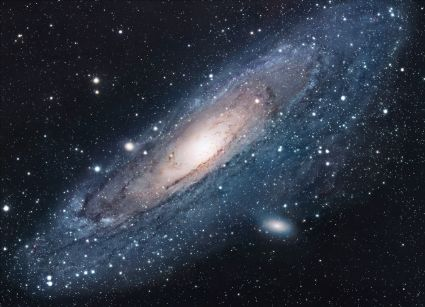
\includegraphics[width=0.5\textwidth]{figures/universe.jpg}
%     \caption{This is an example image}
%     \label{fig:universe}
% \end{figure}

% Do not put any placement constraint on figures,
% such as \texttt{[h]} or \texttt{[h!]}.
% %
% Same considerations apply for other floating elements 
% (e.g. tables, algorithms, listings, etc.).

% Do not use the \texttt{\textbackslash\textbackslash} or \texttt{\textbackslash newline} commands to break lines.

% Just leave an empty line between two paragraphs to start a new one.
% %
% The new line will be automatically indented.
% %
% This is intended: it is the \LaTeX{} way to separate capoverses.

\section{Concept}\label{concept}
This project aims to develop a web-based game application for playing Liar's Poker, a fun and engaging card game centered around deception and bluffing. Inspired by traditional poker, Liar's Poker is played with a standard deck of cards and is suitable for two or more players. Our application will provide an online platform where users can enjoy the game with others in real-time, no matter where they are.

\subsection{Game Rules}\label{game-rules}
Liar's Poker is played with a standard deck of cards without any joker. Each player starts with one card. A round starts with someone naming a poker combination. With the turn rotating clockwise, each next player has a choice:
\begin{itemize}
  \item \textbf{Rise the stakes}\par
  name a higher poker combination than the one named by the previous player that they belive is present in the combined cards of all players.
  \item \textbf{Call bullsh*t} \par
  call bullsh*t on the previous player's combination if the player think the previous player is bluffing or mistaken.
\end{itemize}
When someone calls bullsh*t, all players reveal their cards and the presence of the contested poker hand is verified. If the hand is present, the player who called bullsh*t loses the round; else, the player who named this poker hand loses the round.\par\noindent
The loser starts all subsequent rounds with one extra card, and names the first combination in the next round.\par\noindent
if someone loses when they have 5 cards, they are kicked from the game.
The last person remaining in the game is the winner.

\subsection{Questions and Answers}\label{questions-and-answers}
\begin{itemize}
  \item \textbf{Question:} \emph{How do users interact with the system?}\par
        \textbf{Answer:} Users can access the application through a web browser.
  \item \textbf{Question:} \emph{What happens if one player disconnect during the game?}\par
        \textbf{Answer:} The game will pause until the player reconnects. If the player does not reconnect within a certain time frame, they will be kicked from the game.
  \item \textbf{Question:} \emph{What happens if the server dies during the game?}\par
        \textbf{Answer:} The application goes on, but the game is lost. The players will be redirected to the lobby screen and can choose to play another game or leave the lobby.
  \item \textbf{Question:} \emph{Does the system need to store player's data?}\par
        \textbf{Answer:} The system doesn't need to store data, as the player does not need to create an account.
\end{itemize}
\subsection{Usage Scenarios}\label{usage-scenarios}
This section describes the typical usage scenario of a group of friends playing Liar's Poker on our platform.
\begin{enumerate}
  \item \textbf{Name choice}\par
  The player chooses a nickname to use during the game.
  \item \textbf{Lobby creation}\par
  One user creates a new lobby and share the access code with friends. 
  \item \textbf{Joining the lobby}\par
  Other users join the lobby by entering the code.
  \item \textbf{Gameplay}\par
  Each player receive one card and than the game starts. The game proceeds as described in the rules. when the player want to rise the stakes, he can choose from the possible combinations (non valid combinations will be disabled), if the combination needs some specific rank or suit to be declared, the player will be provided with a list of possible ones to choose from.
  \item \textbf{Elimination}\par
  When a player loses, they are eliminated from the game.
  \item \textbf{End of the game}\par
  When the game ends the winner is declared and players will be redirected to the lobby page where they can choose to play another game or leave the lobby.
\end{enumerate}

% create a figure with 3 images
\begin{figure}[H]
  \centering
  \subfloat[Home and Lobby Selection]{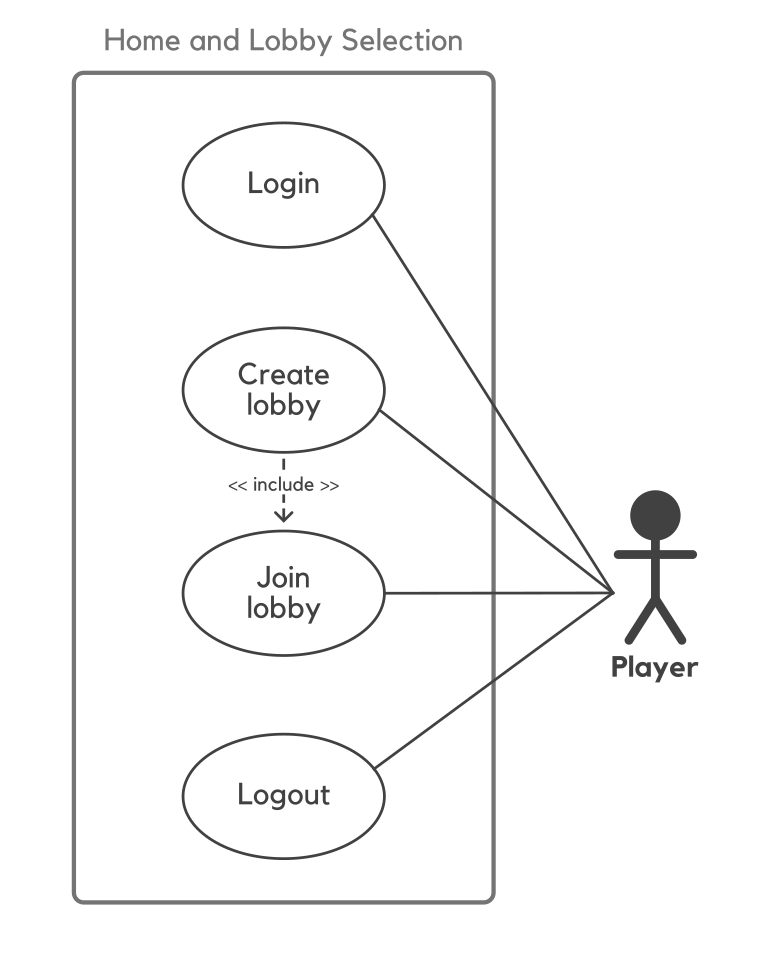
\includegraphics[width=0.5\textwidth]{figures/homeLobbyUseCase.png}}
  \hfill
  \subfloat[Lobby]{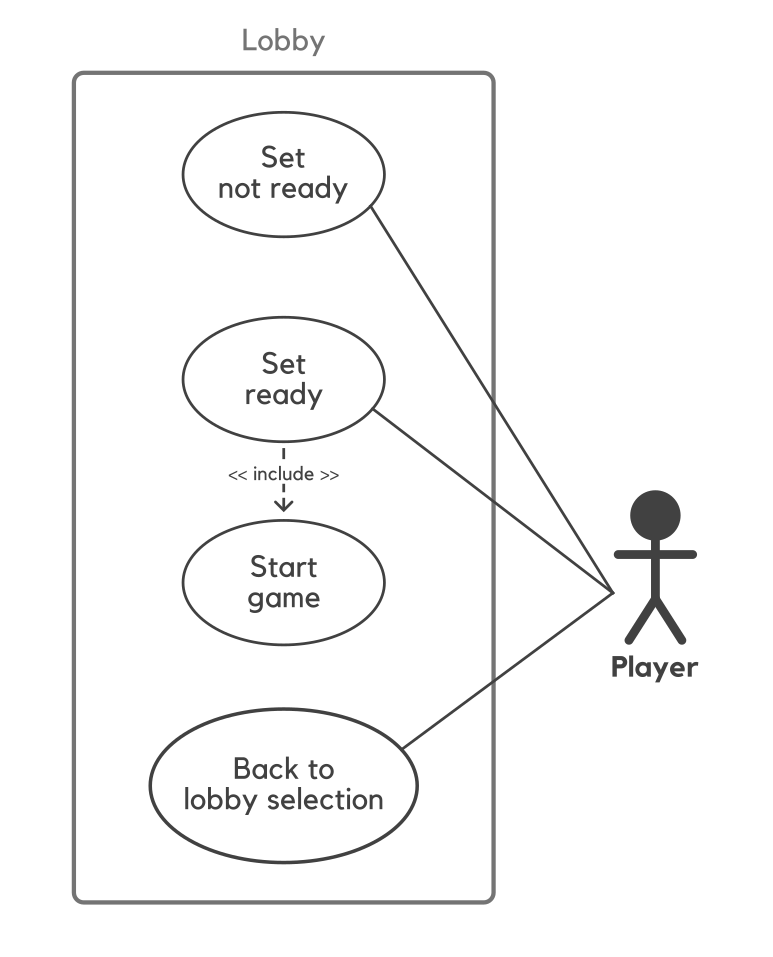
\includegraphics[width=0.5\textwidth]{figures/lobbyUseCase.png}}
  \hfill
  \subfloat[Match]{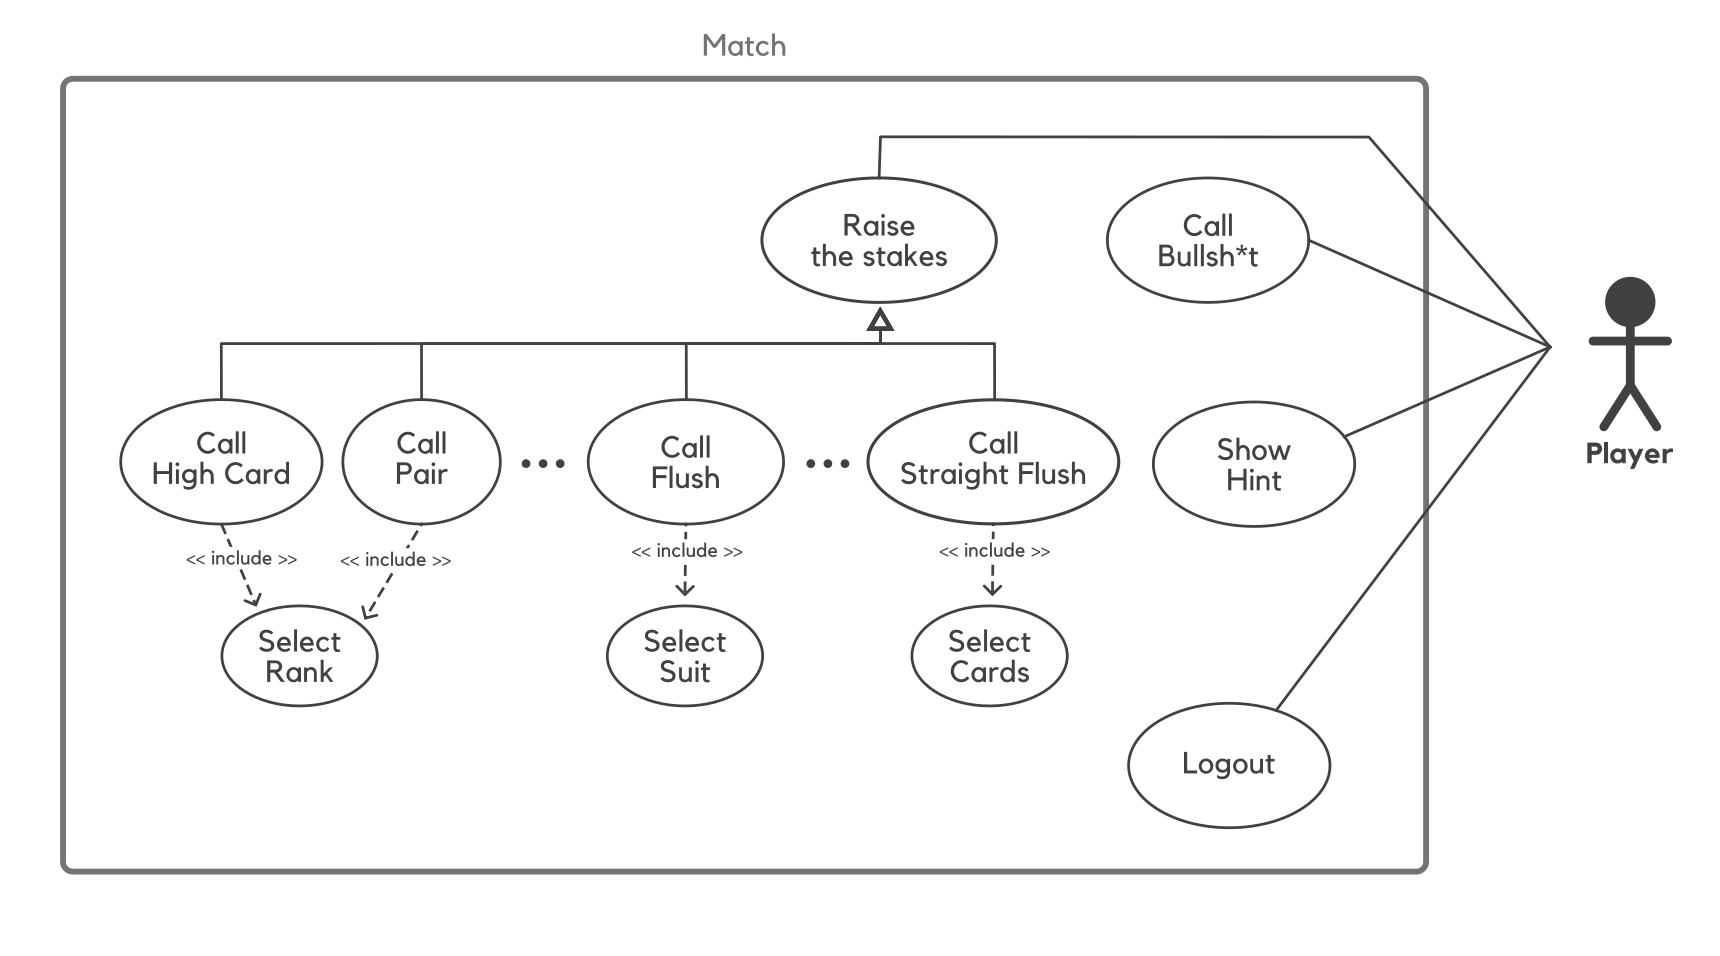
\includegraphics[width=1\textwidth]{figures/gameUseCase.png}}
  \caption{Use Case Diagrams}
\end{figure}

\begin{comment}
Here you should explain:

\begin{itemize}
  \item The type of product developed with that project, for example
  (non-exhaustive):

  \begin{itemize}
    \item Application (with GUI, be it mobile, web, or desktop)
    \item Command-line application (CLI could be used by humans or scripts)
    \item Library
    \item Web-service(s)
  \end{itemize}
  \item Use case collection

  \begin{itemize}
    \item \emph{where} are the users?
    \item \emph{when} and \emph{how frequently} do they interact with the
    system?
    \item \emph{how} do they \emph{interact} with the system? which
    \emph{devices} are they using?
    \item does the system need to \emph{store} user's \textbf{data}?
    \emph{which}? \emph{where}?
    \item most likely, there will be \emph{multiple} \textbf{roles}
  \end{itemize}
\end{itemize}
\end{comment}

\section{Requirements}\label{requirements}
Starting from the concept, we can identify the following requirements for the application:
\subsection{Functional Requirements}\label{functional-requirements}
\begin{enumerate}
  \item \textbf{Lobby Creation}\par
  The application must allow users to create a new lobby and share the access code with friends.
  \item \textbf{Lobby Joining}\par
  The application must allow users to join a lobby by entering the access code.
  \item \textbf{Gameplay}\par
  The application must allow users to play Liar's Poker following the game rules.
\end{enumerate}

\subsection{Non-functional Requirements}\label{non-functional-requirements}
\begin{enumerate}
  \item \textbf{Scalability}\par
  The application must be able to handle multiple lobbies and games simultaneously.\par
  \begin{itemize}
    \item \textbf{Acceptance Criteria:} The system must be able to handle at least 5 concurrent games.
  \end{itemize}
  \item \textbf{Fault Tollerance}\par
  The application must be able to handle user disconnections without losing a running game and should recover from server failures. 
  \begin{itemize}
    \item \textbf{Acceptance Criteria:} The system must be able to recover from server failures within 1 minute.
  \end{itemize}
  \item \textbf{Consistency}\par
  The application must ensure that all players see the same game state at all times.
  \begin{itemize}
    \item \textbf{Acceptance Criteria:} The system must ensure that all players see the same game state within 1 second from the bullsh*t call.
  \end{itemize}
  \item \textbf{Performance}\par
  The application must be able to have good response times.
  \begin{itemize}
    \item \textbf{Acceptance Criteria:} A new game must be created within 5 seconds.
  \end{itemize}
  

\end{enumerate}

\subsection{Glossary of cards combinations}\label{cards-combinations}  
in this section we list all the possible cards combinations, that can be declared during the game, ordered by increasing value:
\begin{enumerate}
  \item \textbf{High Card}\par
  in the combined cards of all players there is a card with the rank declared by the player.
  \item \textbf{Pair}\par
  in the combined cards of all players there are two cards with the same rank declared by the player.
  \item \textbf{Two Pair}\par
  in the combined cards of all players there are two pairs of cards with the same ranks declared by the player.
  \item \textbf{Three of a Kind}\par
  in the combined cards of all players there are three cards with the same rank declared by the player.
  \item \textbf{Straight}\par
  in the combined cards of all players there are five cards with consecutive values declared by the player.
  \item \textbf{Flush}\par
  in the combined cards of all players there are five cards with the same suit declared by the player.
  \item \textbf{Full House}\par
  in the combined cards of all players there is a \emph{pair} and a \emph{three of a kind} with the respective ranks declared by the player. 
  \item \textbf{Four of a Kind}\par
  in the combined cards of all players there are four cards with the same value declared by the player.
  \item \textbf{Straight Flush}\par
  in the combined cards of all players there are five cards with consecutive values and the same suit declared by the player.
  \item \textbf{Royal Flush}\par
  in the combined cards of all players there are five cards with the same suit declared by the player and the ranks \emph{10}, \emph{J}, \emph{Q}, \emph{K} and \emph{Ace}.
\end{enumerate}

\begin{comment}
\begin{itemize}
  \item The requirements must explain \textbf{what} (not how) the software
  being produced should do.

  \begin{itemize}
    \item you should not focus on the particular problems, but exclusively on
    what you want the application to do.
  \end{itemize}
  \item Requirements must be clearly identified, and possibly numbered
  \item Requirements are divided into:

  \begin{itemize}
    \item \textbf{Functional}: some functionality the software should provide
    to the user
    \item \textbf{Non-functional}: requirements that do not directly concern
    behavioural aspects, such as consistency, availability, etc.
    \item \textbf{Implementation}: constrain the entire phase of system
    realization, for instance by requiring the use of a specific
    programming language and/or a specific software tool

    \begin{itemize}
      \item these constraints should be adequately justified by political /
      economic / administrative reasons\ldots{}
      \item \ldots{} otherwise, implementation choices should emerge \emph{as
      a consequence of} design
    \end{itemize}
  \end{itemize}
  \item If there are domain-specific terms, these should be explained in a
  glossary
  \item Each requirement must have its own \textbf{acceptance criteria}

  \begin{itemize}
    \item these will be important for the validation phase
  \end{itemize}
\end{itemize}
\end{comment}

\section{Design}\label{design}

This chapter explains the strategies used to meet the requirements
identified in the analysis. Ideally, the design should be the same,
regardless of the technological choices made during the implementation
phase.

\begin{quote}
You can re-order the sections as you prefer, but all the sections must
be present in the end
\end{quote}

\subsection{Architecture}\label{architecture}

  The architecture of the system is a classic MVC where:
  \begin{itemize}
    \item Model are the classes that represents players and cards
    \item View is UI realized with Web components
    \item Controller is the class that manages the game logic
  \end{itemize}
  For the communication architecture and the distributed part, we opted for a client-server architecture using also a publish-subscribe pattern. \newline
  The idea is that the broker manages the communication between the clients and the server, and the server manages the game logic.\newline
  The server is the one that creates the game; then the clients can join the game publishing their nickname to the broker; every time a new player joins the game, it automatically subscribe to the game topics.\newline
  All the clients are subscribed to the same topic, so they can receive the messages from the server (eg. moves, game status, etc.).\newline

  We choose this architecture because it is simple and it is suitable for our project. In fact, using a publish-subscribe architecture, clients have not to request the server for the game status, but they receive it automatically when the server publishes it (and so on for the other messages).

\subsection{Infrastructure}\label{infrastructure}

  \begin{itemize}
    \item both players and server are components of the pub-sub model
    \item there is one server that manages the game logic so is the only one who can publish messages on some specific topics
    \item there is a broker that manages the communication between the clients and the server
    \item data aren't store permanently, so there is no need for a database 
    \item there aren't authentication mechanisms so every one who knows the broker address can join the game

  \end{itemize}
  Components are distributed over all the network, so they can be on different machines and different networks. For semplicity, we used the same network for all the components and the same machine both for server and broker. \newline
  To find each other, the components use the broker address and the topics to which they have to subscribe or publish; so clients are only required to know the broker address to join the game. \newline
  Components are named using a unique nickname that every body choose on game launch.


\begin{figure}[H]
  \caption{Architecture diagram}
  \centering
  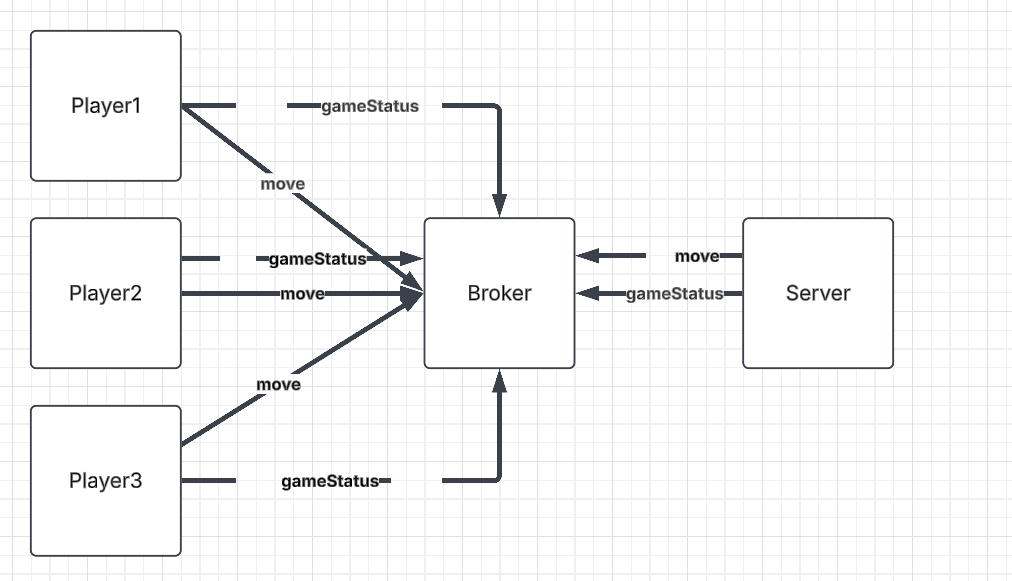
\includegraphics[scale=0.5]{figures/pubsubdiagram.png}
  \end{figure}

  Dotted lines are for subscribe messages, while solid lines are for publish messages. \newline

\subsection{Modelling}\label{modelling}
% \begin{itemize}
%   \item which \textbf{domain entities} are there?

%   \begin{itemize}
%     \item e.g.~\emph{users}, \emph{products}, \emph{orders}, \emph{etc.}
%   \end{itemize}
%   \item how do \emph{domain entities} \textbf{map to} \emph{infrastructural
%   components}?

%   \begin{itemize}
%     \item e.g.~state of a video game on central server, while
%     inputs/representations on clients
%     \item e.g.~where to store messages in an IM app? for how long?
%   \end{itemize}
%   \item which \textbf{domain events} are there?

%   \begin{itemize}
%     \item e.g.~\emph{user registered}, \emph{product added to cart},
%     \emph{order placed}, \emph{etc.}
%   \end{itemize}
%   \item which sorts of \textbf{messages} are exchanged?

%   \begin{itemize}
%     \item e.g.~\emph{commands}, \emph{events}, \emph{queries}, \emph{etc.}
%   \end{itemize}
%   \item what information does the \textbf{state} of the system comprehend

%   \begin{itemize}
%     \item e.g.~\emph{users' data}, \emph{products' data}, \emph{orders' data},
%     \emph{etc.}
%   \end{itemize}
% \end{itemize}

% \begin{quote}
% Class diagram are welcome here
% \end{quote}
The system is foundamentally composed by the classes shown in \cref{fig:classes}. \newline
Each component models the real world entities that are needed to play the game in a non-distributed
way, this are the classes that the controller will later use to make the game work.
\begin{figure}[H]
  \centering
  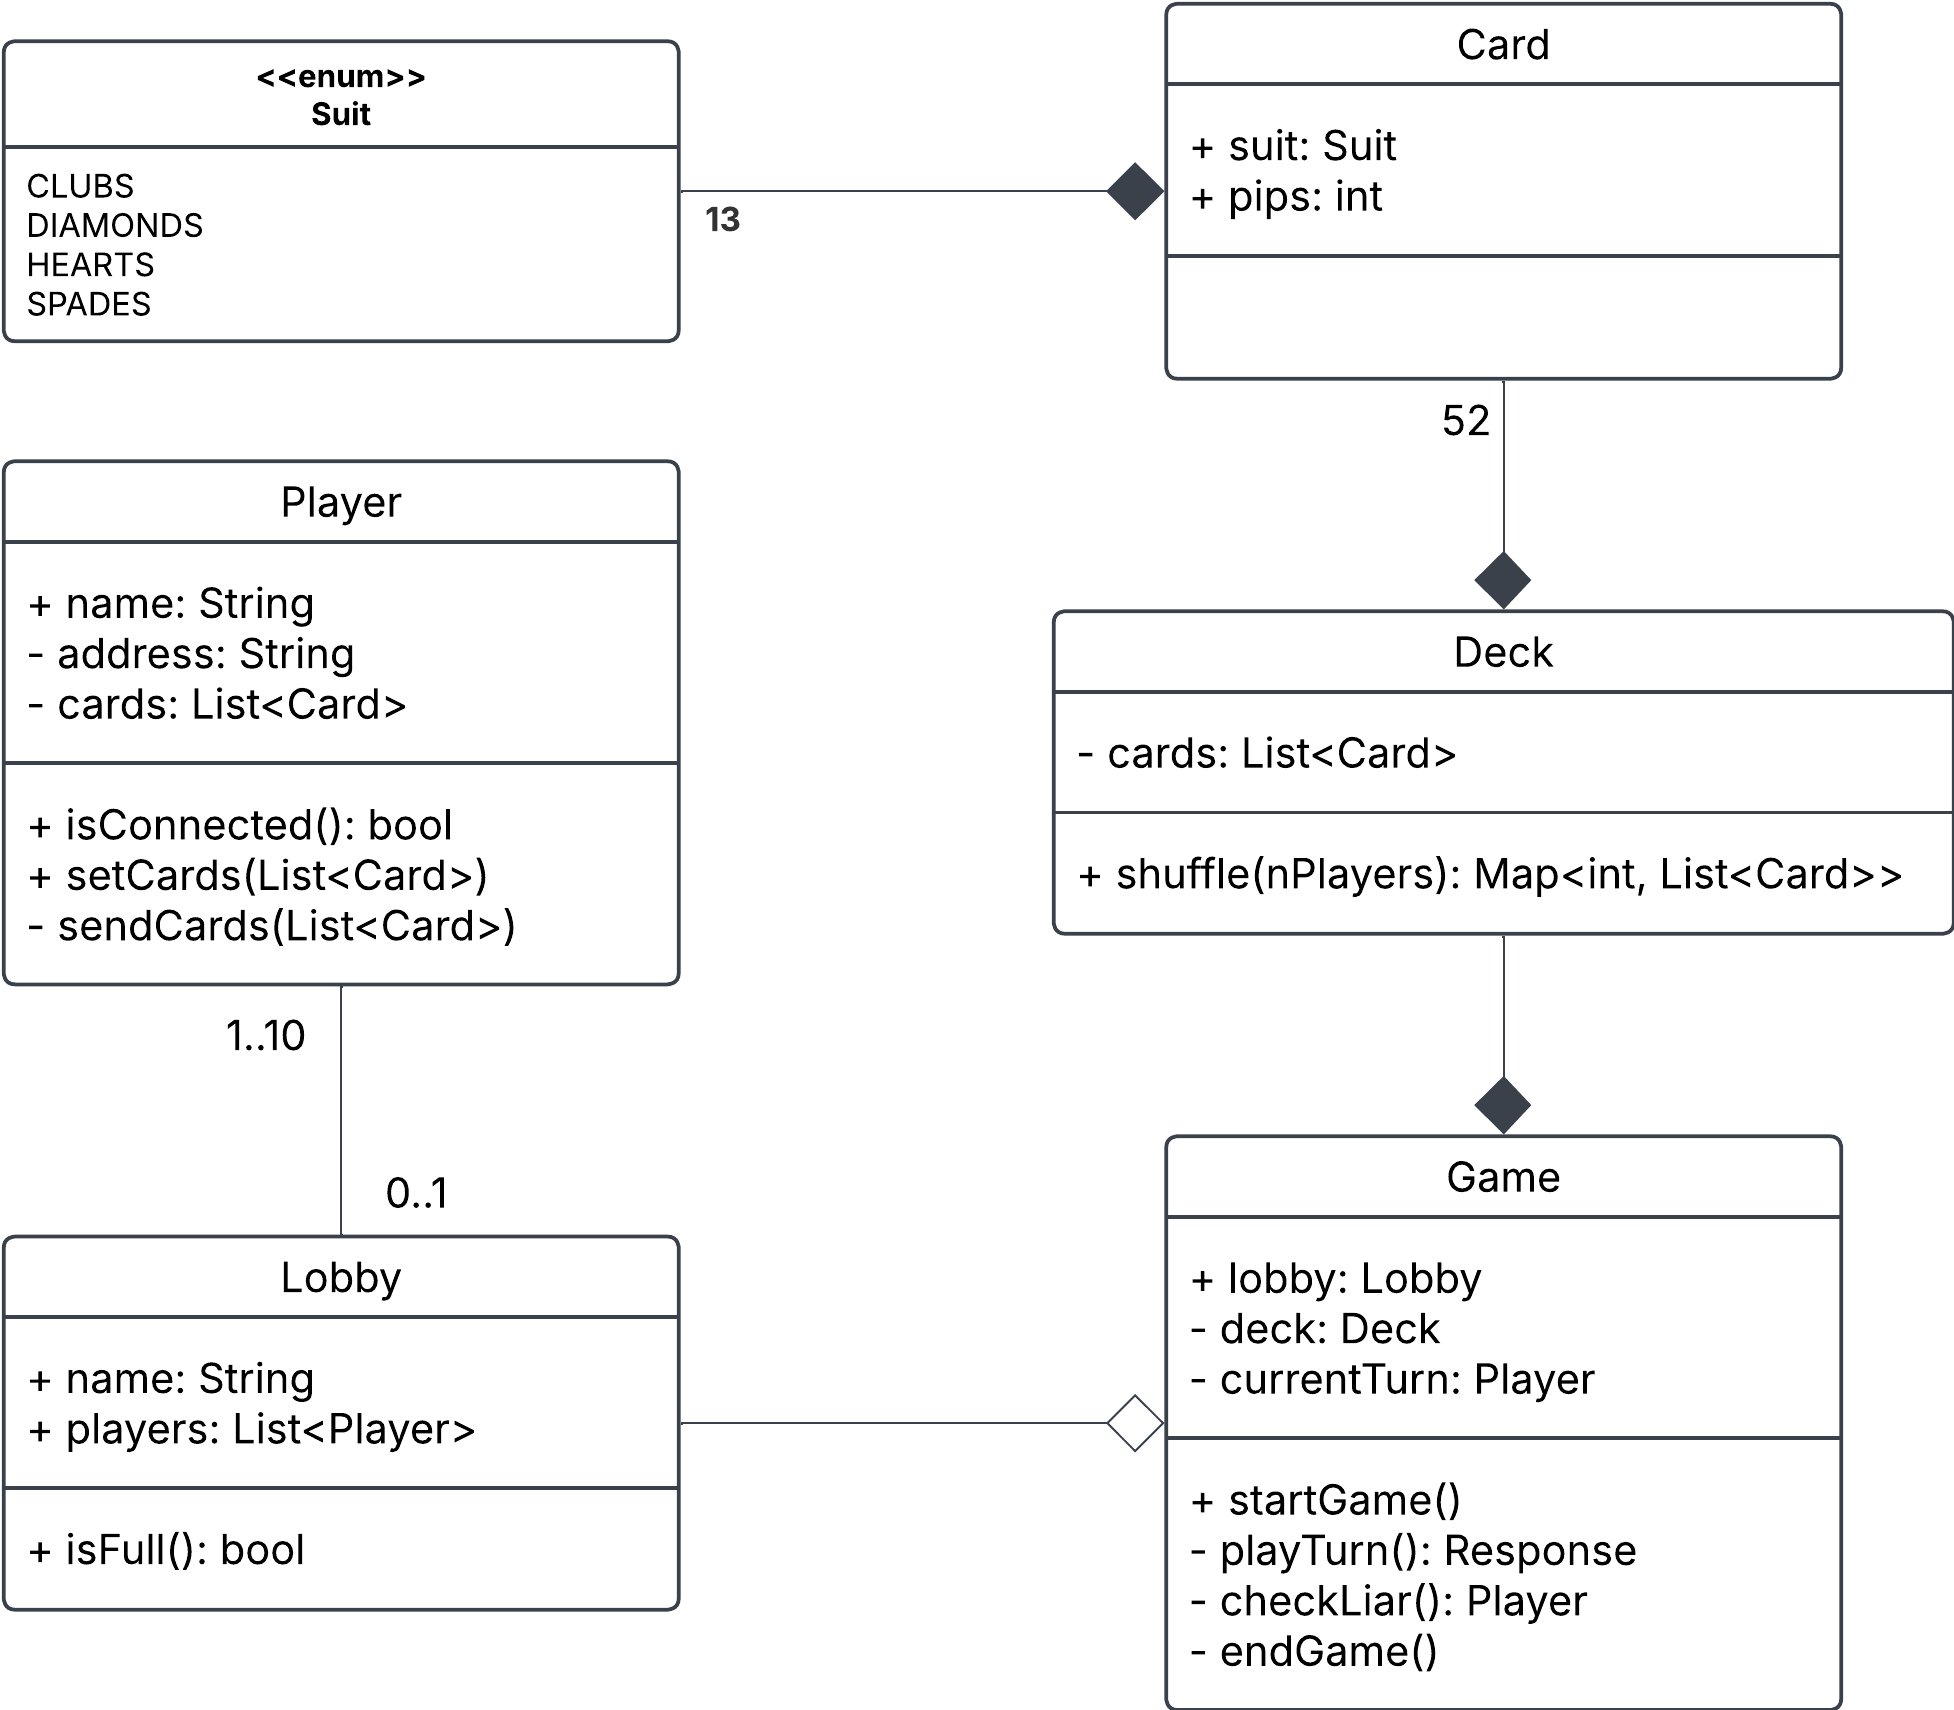
\includegraphics[width=0.8\textwidth]{figures/classes.png}
  \caption{Class diagram of the system} 
  \label{fig:classes}
\end{figure}

The game is the most important entity of the whole model. It has a deck of cards, that can be shuffled,
and a set of players, each one with a nickname and his given cards. 
To handle the game logic it keeps in memory the current player and the latest raise. \newline
It can be asked to:
\begin{itemize}
  \item Add or remove a player from the game
  \item Get a fresh set of shuffled cards for the players
  \item Raise the stakes and advance the turn
  \item Check if the latest stake was a lie
  \item Get the currently playing user
  \item Get the player that raised the stakes
\end{itemize}

At the core of the entire system are messages, these, given the simple nature of the game, are quite 
simple: containing a single string that represents the move the player wants to make. \newline
The real difference and context of the message is given by the topic to which it is published: 
ff a name is passed to the "player" topic it will be interpreted as the player's nickname,
if it is passed to the "game" topic it will be interpreted as the player's move. \newline
Most notably these are the main topics:
\begin{itemize}
  \item \textbf{player} \par
  The topic where the players publish their nickname to join the game.
  \item \textbf{game} \par
  The topic where the players publish their moves and the server the game status. \newline
  The name of the topic varies depending on the lobby the player is in.
  \item \textbf{lobby} \par
  The topic where the players create and join lobbies.
\end{itemize}

\subsection{Interaction}\label{interaction}

Components communicate over the network using the MQTT protocol so using a Message Broker pattern. Using this pattern, publishers can send messages without knowing who is going to receive them, and subscribers can receive messages without knowing who is going to send them. 
The broker is the one who manages the communication between the clients and the server, so the clients don't have to know the server address, but only the broker address; on the other hand, the server has to know the broker address to publish messages, but it doesn't have to know the clients' addresses. \newline
This kind of architecture is highly decoupled, so the components can be easily replaced or modified without affecting the others. \newline
The following subsections will explain the interaction between the components in more detail.

\subsubsection{Connection}\label{connection}
\begin{figure}[H]
  \centering
  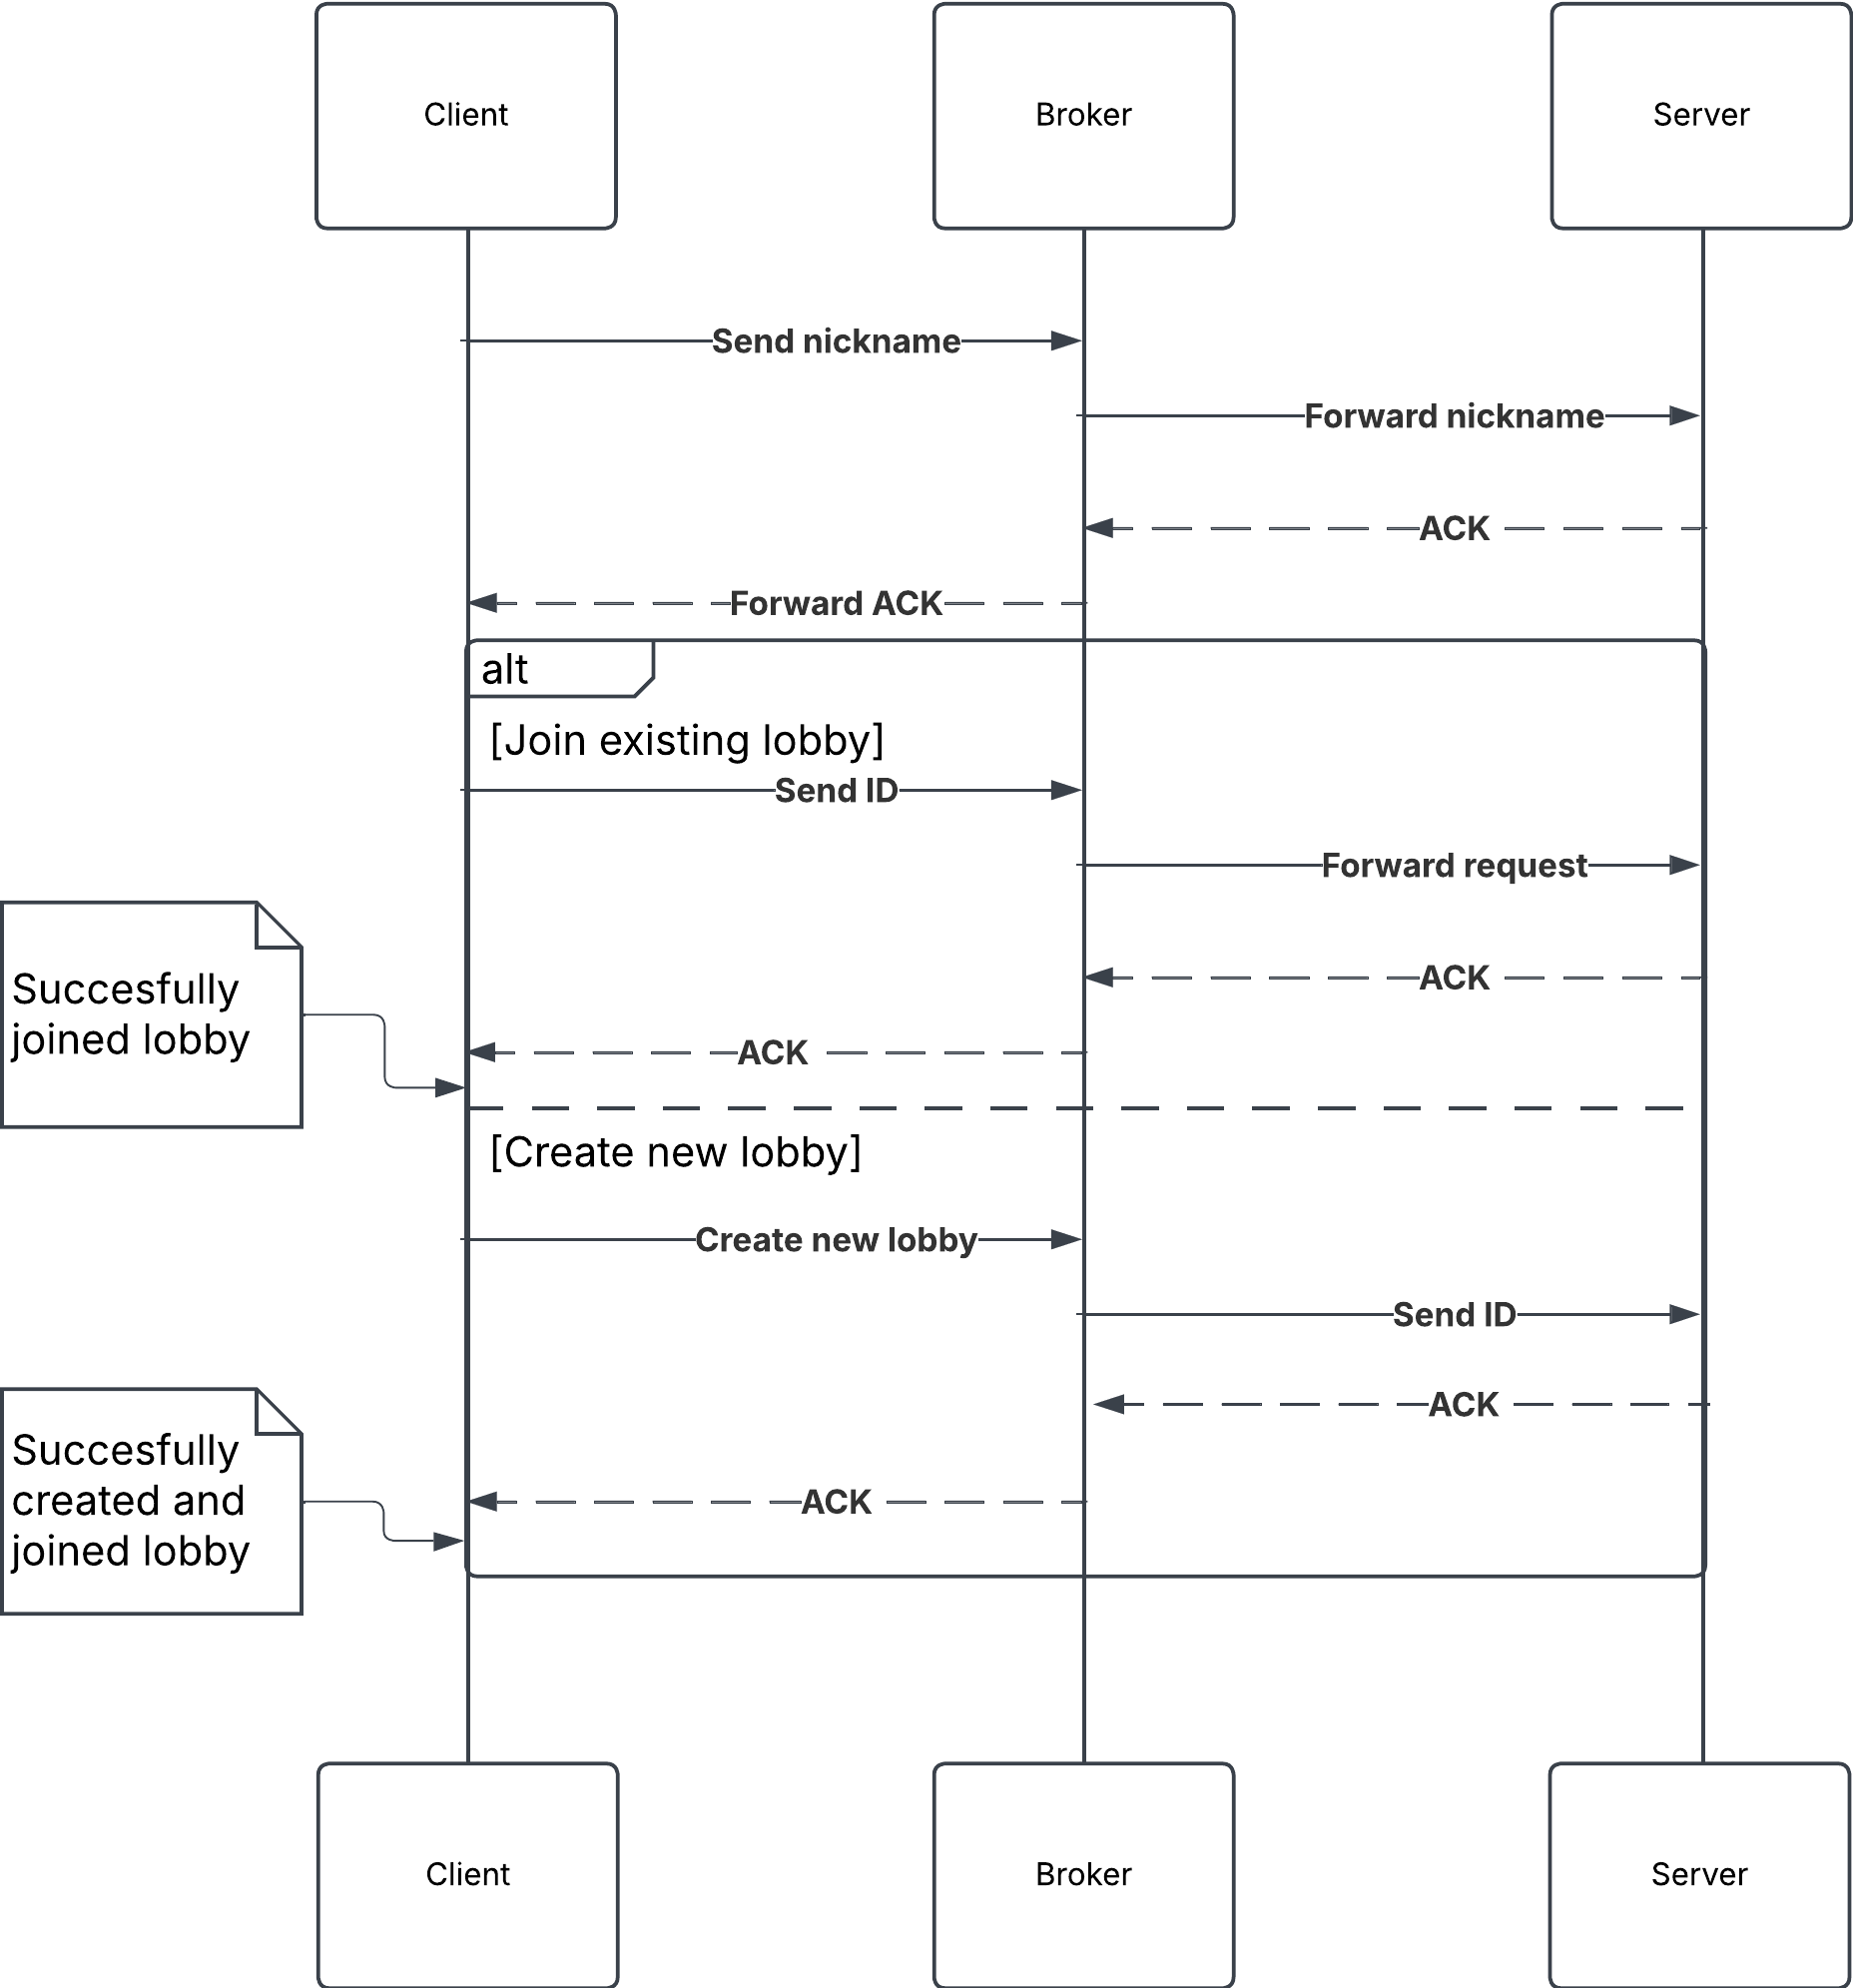
\includegraphics[width=0.8\textwidth]{figures/sequenceConnection.png}
  \caption{Sequence diagram of the connection phase} 
  \label{fig:connection}
\end{figure}

\subsubsection{Game Move}\label{game-move}
\begin{figure}[H]
  \centering
  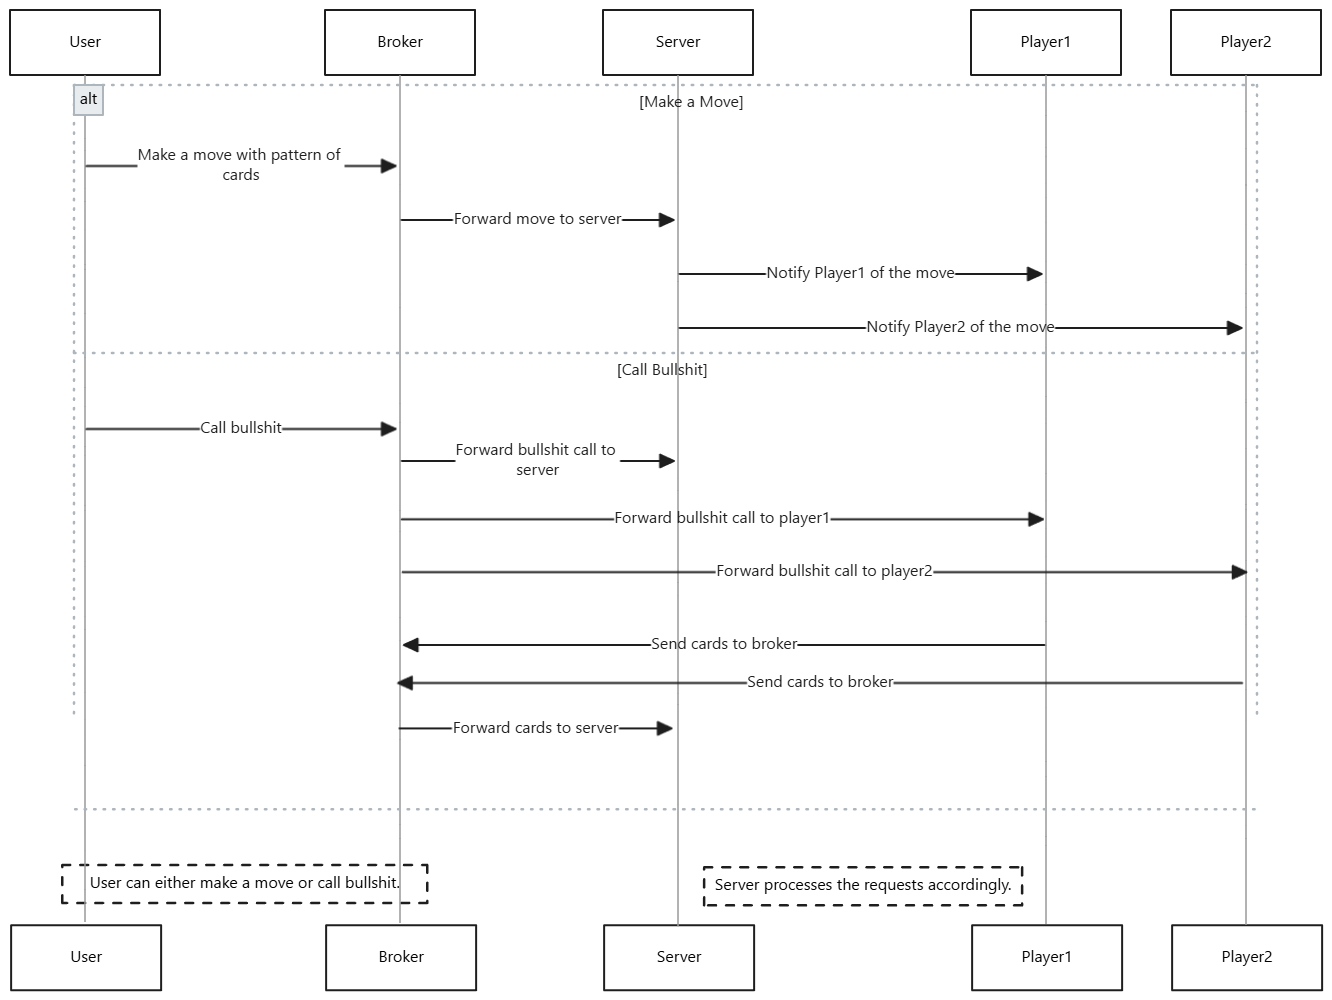
\includegraphics[width=0.8\textwidth]{figures/sequenceGameMove.png}
  \caption{Sequence diagram of a generic game move} 
  \label{fig:gane-move}
\end{figure}

\subsubsection{End Game}\label{end-game}
\begin{figure}[H]
  \centering
  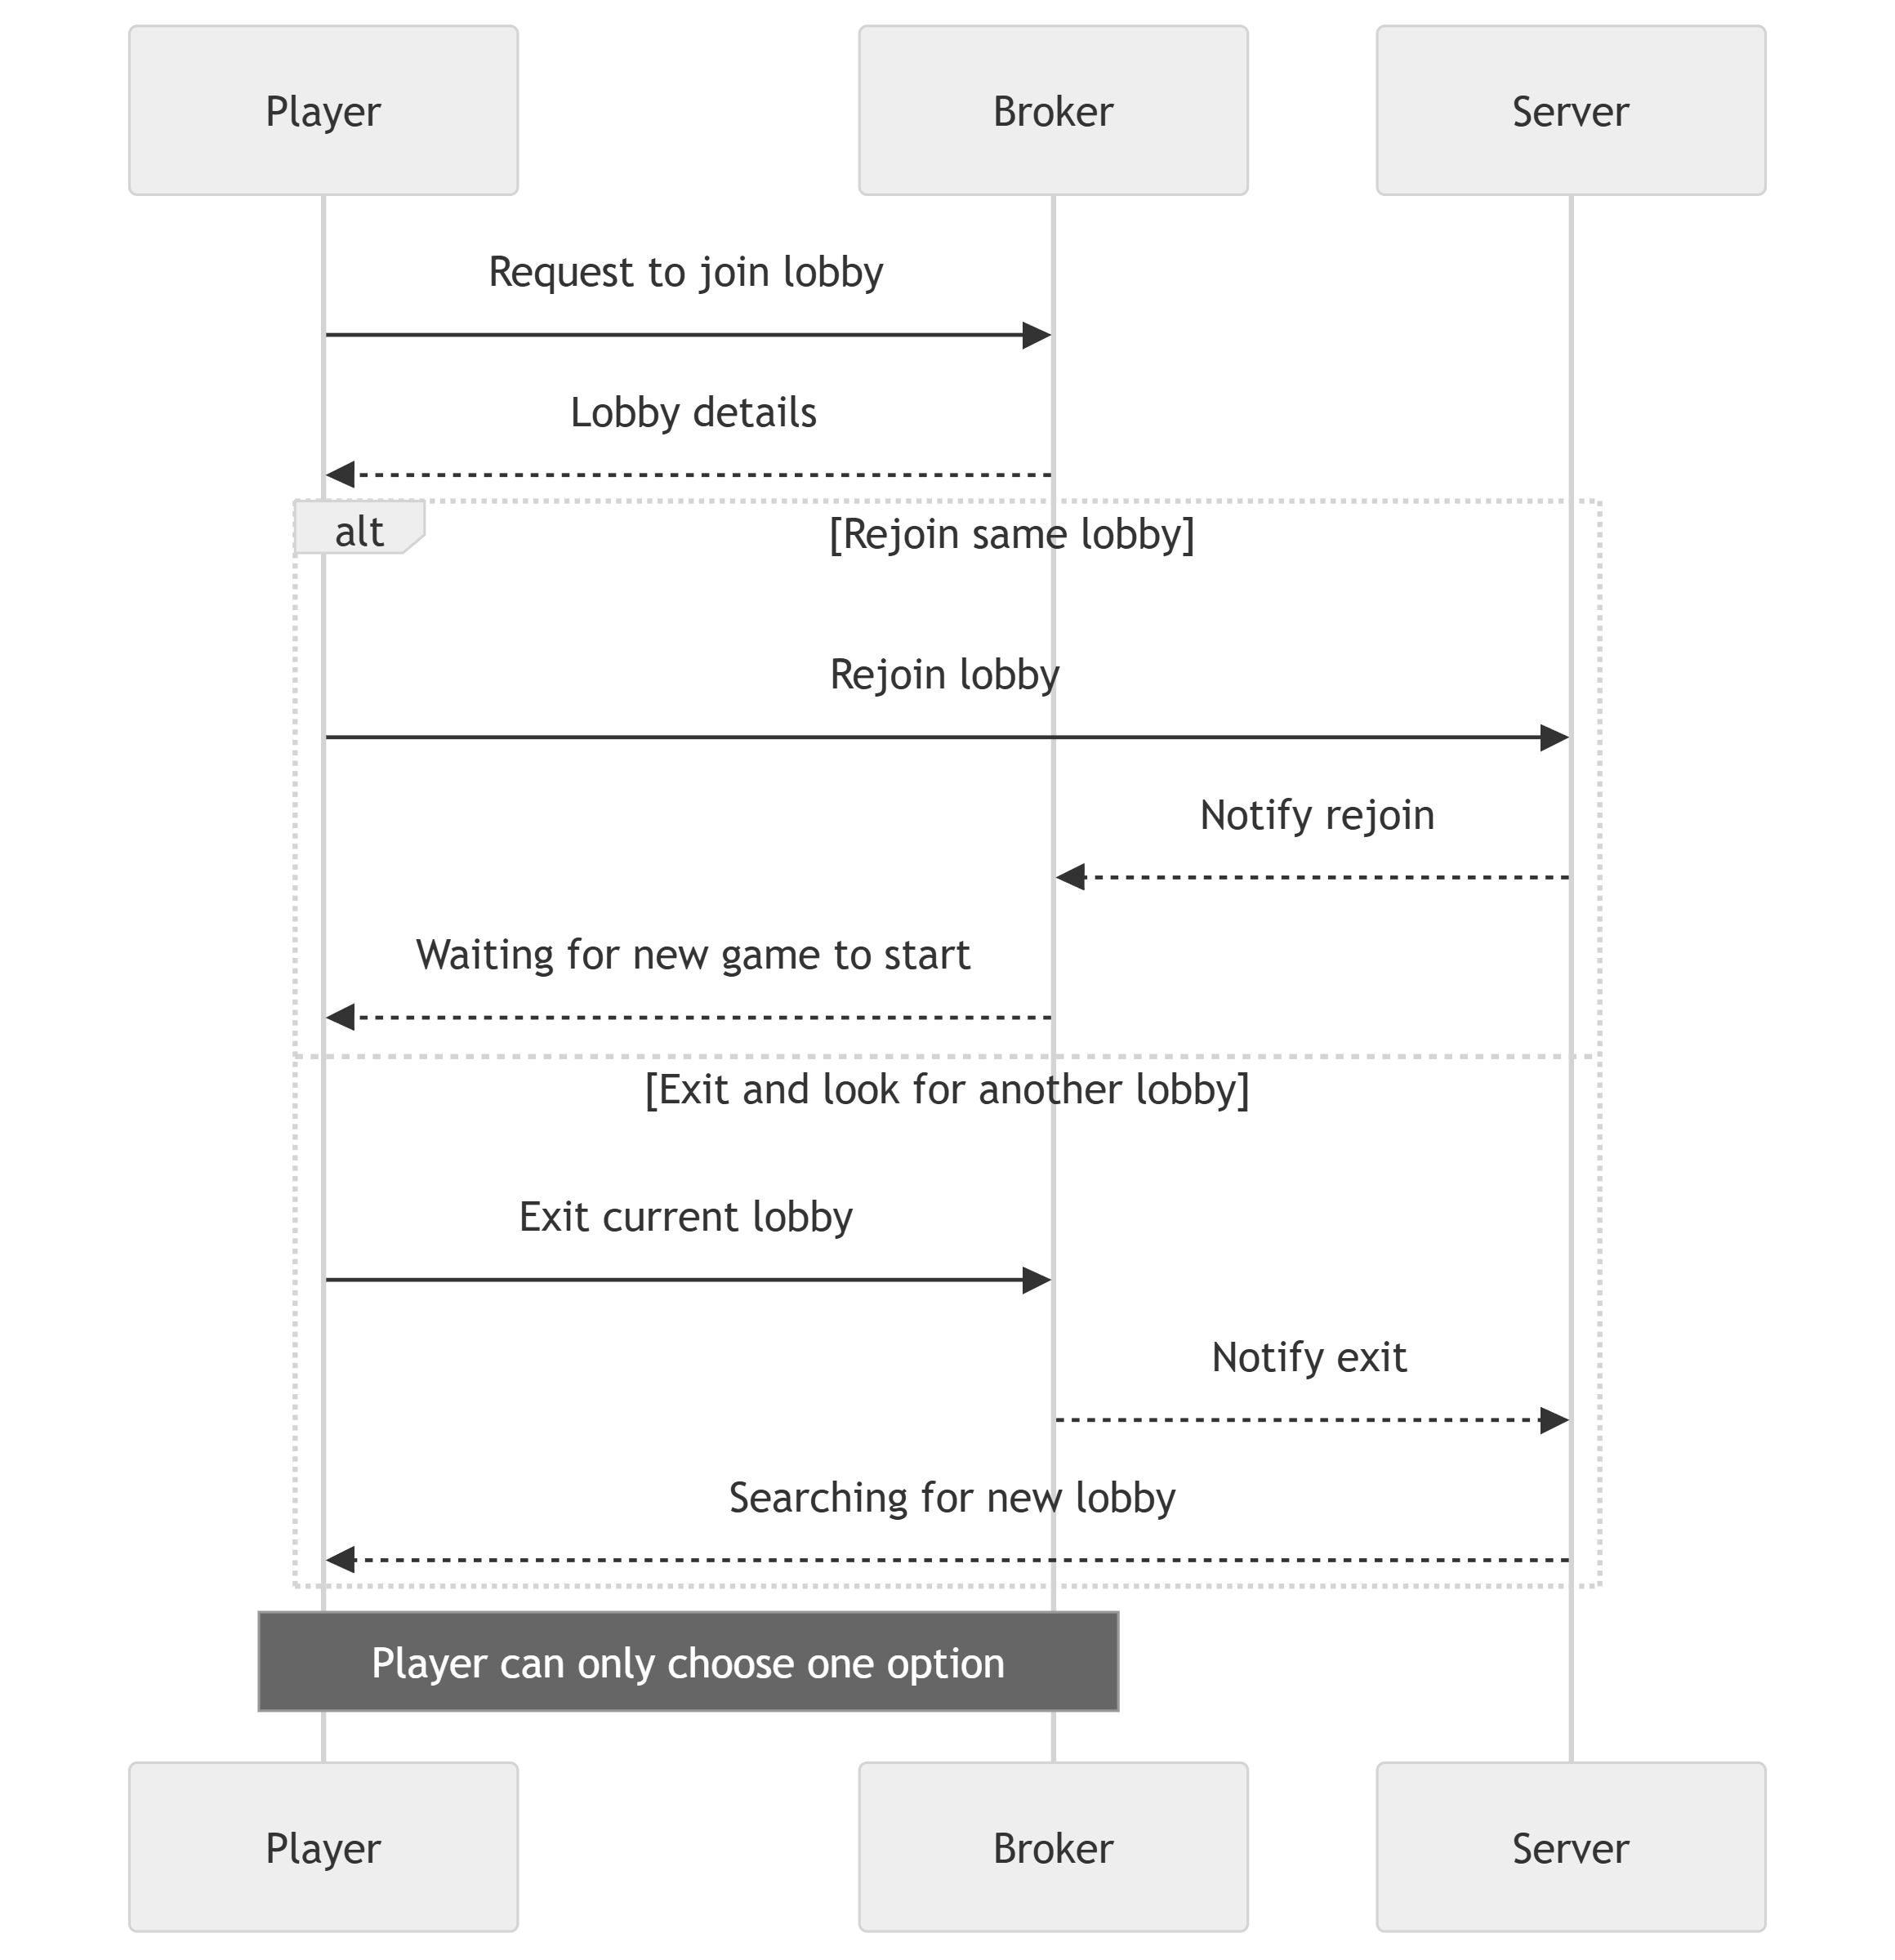
\includegraphics[width=0.8\textwidth]{figures/sequenceEndGame.png}
  \caption{Use case diagram of end game phase} 
  \label{fig:end-game}
\end{figure}


\subsection{Behaviour}\label{behaviour}
% \begin{itemize}
%   \item how does \emph{each} component \textbf{behave} individually (e.g.~in
%   \emph{response} to \emph{events} or messages)?

%   \begin{itemize}
%     \item some components may be \emph{stateful}, others \emph{stateless}
%   \end{itemize}
%   \item which components are in charge of updating the \textbf{state} of the
%   system? \emph{when}? \emph{how}?
% \end{itemize}

% \begin{quote}
% State diagrams are welcome here
% \end{quote}
Even if for the game to be played are only needed players and a centralized logic,
more actors are needed to keep the game going and to manage the communication between them. \newline
The following are all the components actually needed and their behaviours:
\begin{itemize}
  \item
  \textbf{The client} \cref{fig:clientStates} \par
  The client first asks the player for their name and the tries to connect him to the broker. 
  If the connection is successful, the client can choose to join a lobby or create a new one. \newline
  When the game starts, the client waits for the server to publish the game status and then it can start playing.
  The client can only send messages to the server when it is his turn, either rising the stakes 
  or calling bullsh*t. If they player lost the match can only wait for it to finish.
  The player leaves the lobby only when a winner is found or loses the game. When the game ends the
  player can rejoin the same lobby and wait for a new game to start or look for a new one. \newline
  At any point during the connection the player can leave or be disconnected, if the player wants to rejoin
  the system will try to put him back in a lobby if they where in one.
  \begin{figure}[H]
    \centering
    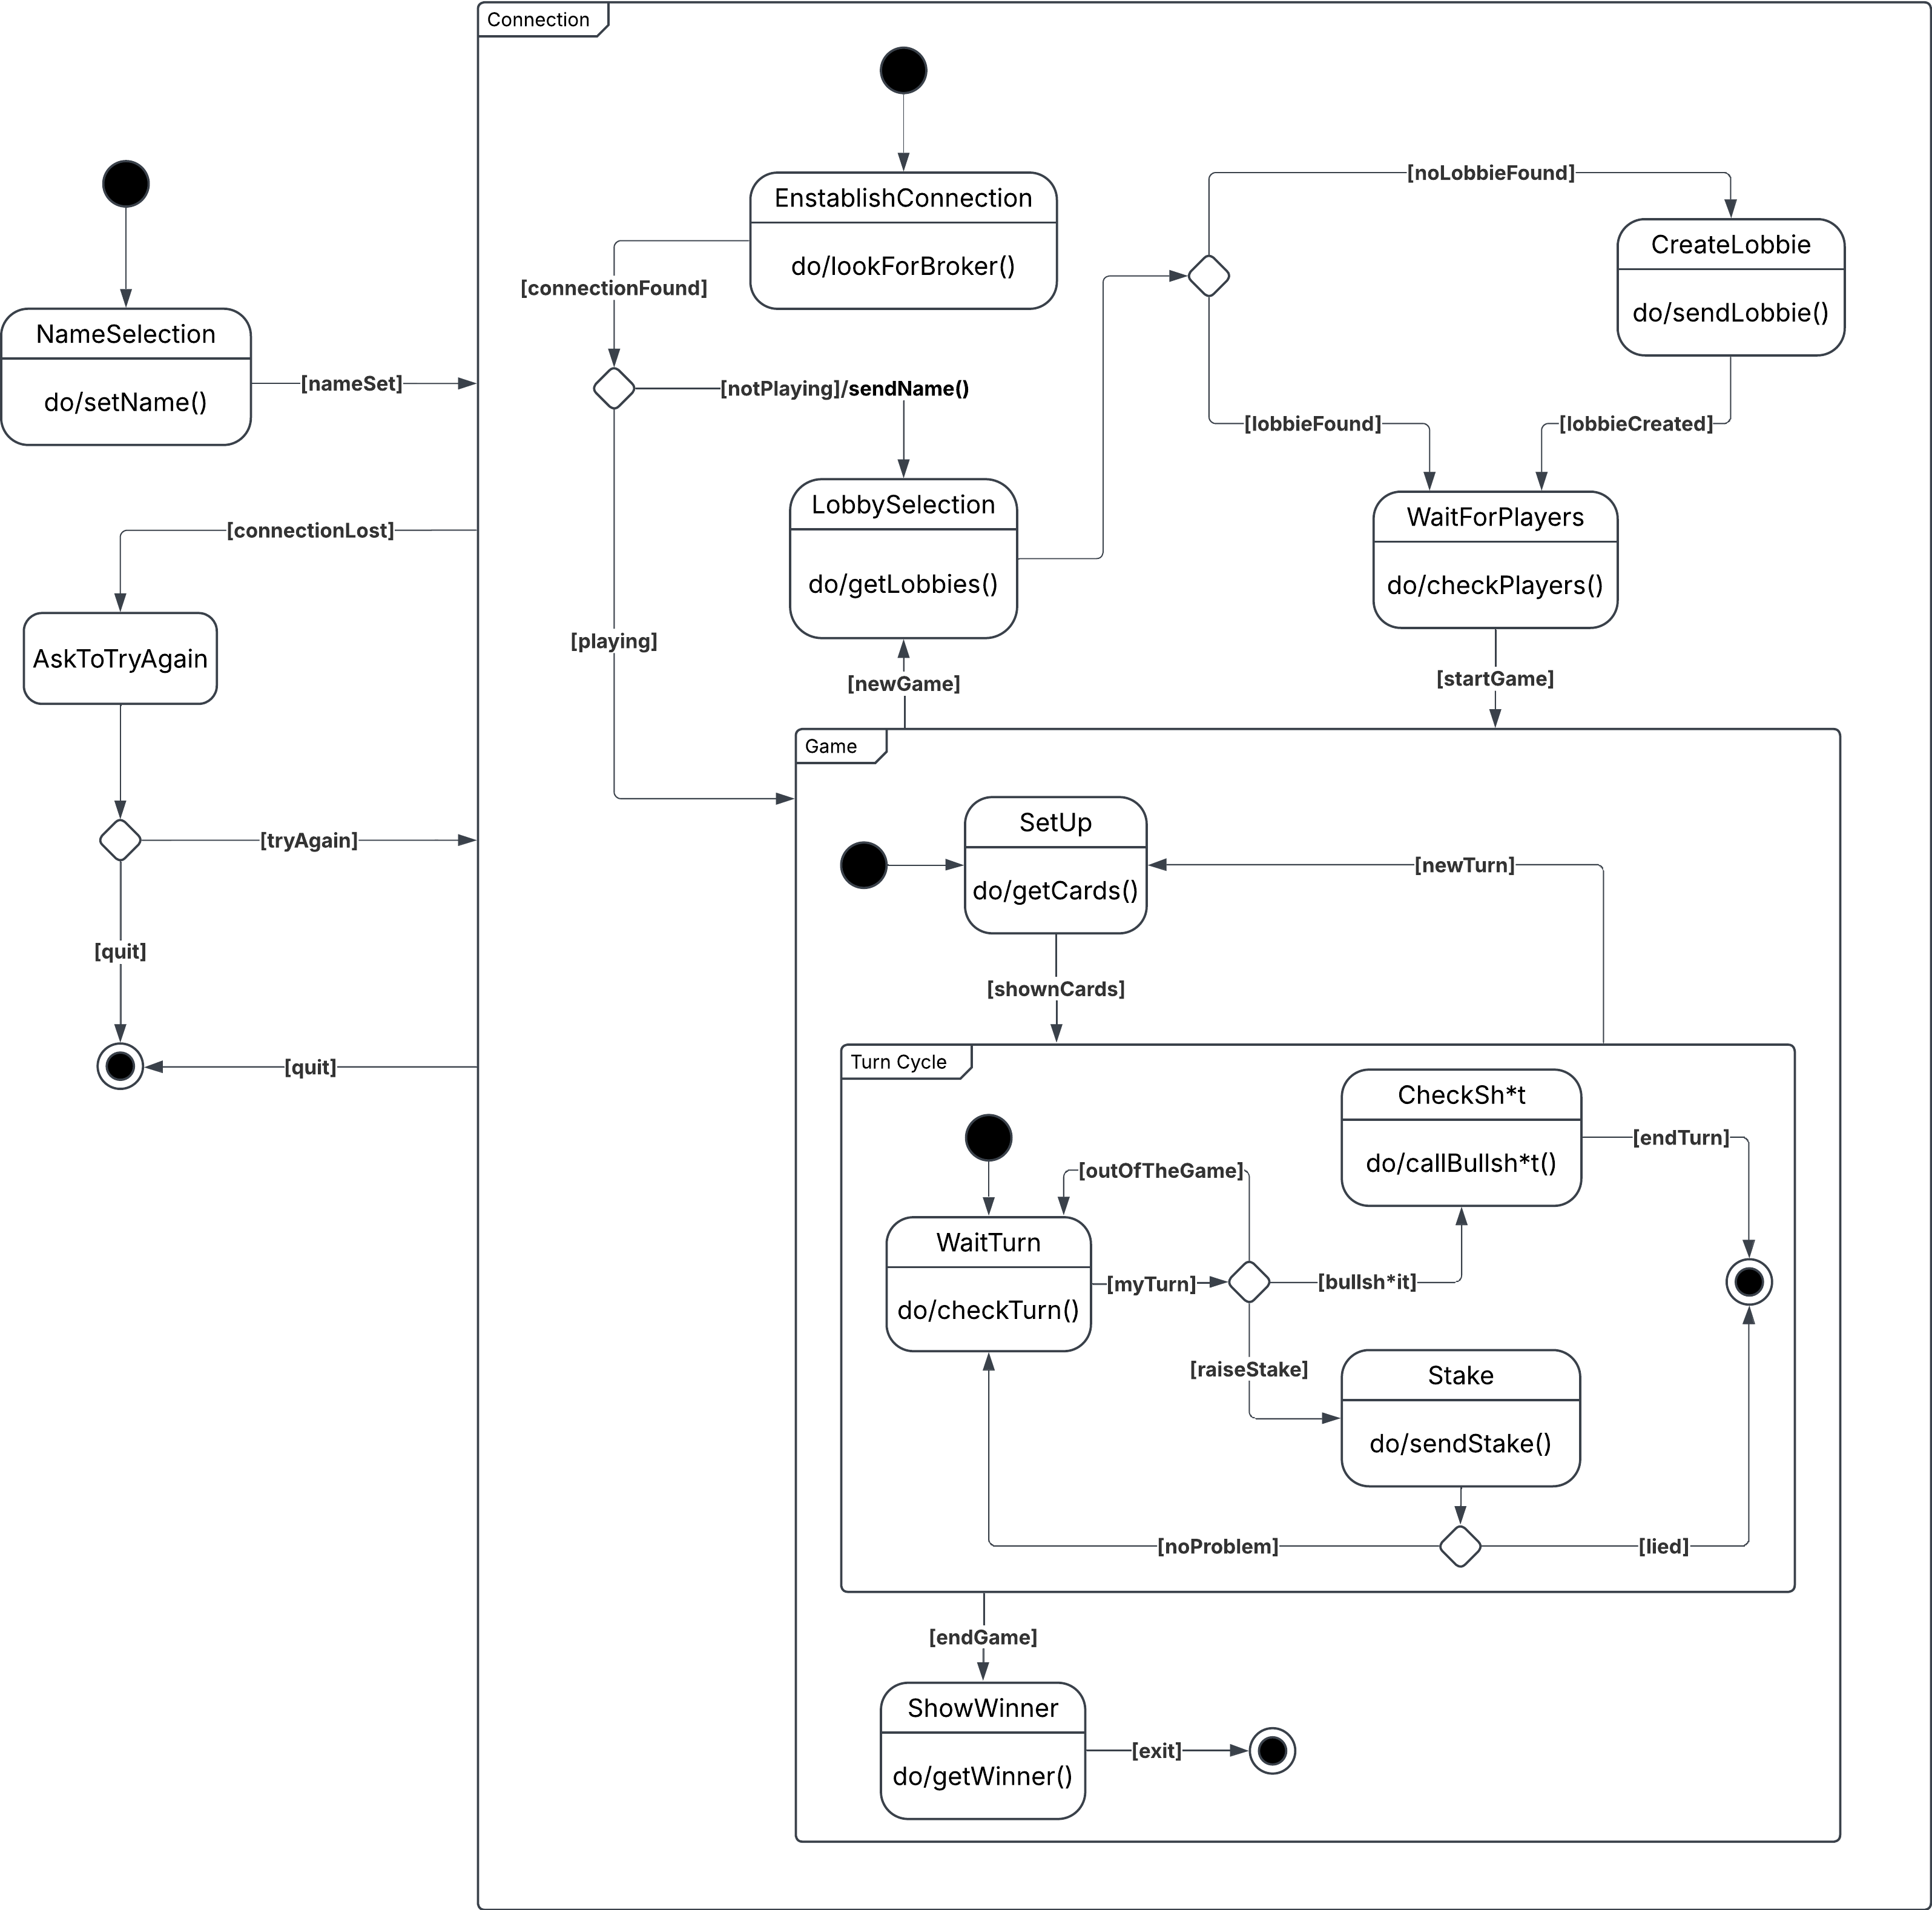
\includegraphics[width=0.8\textwidth]{figures/clientStates.png}
    \caption{State diagram of the client} 
    \label{fig:clientStates}
  \end{figure}
  \item
  \textbf{The server} \cref{fig:serverStates} \par
  The server is mainly in charge of connecting new players and creating lobbies, 
  delegating the game logic to an agent. \newline
  At any point in time a new player can ask to connect or disconnect himself, causing the need to
  check wether the player was alone in a lobby, deleting it if left empty. The players connected 
  can also ask to create or join a new lobby and, in case it's full or closed by a player, 
  it will launch a new game istance.
  \begin{figure}[H]
    \centering
    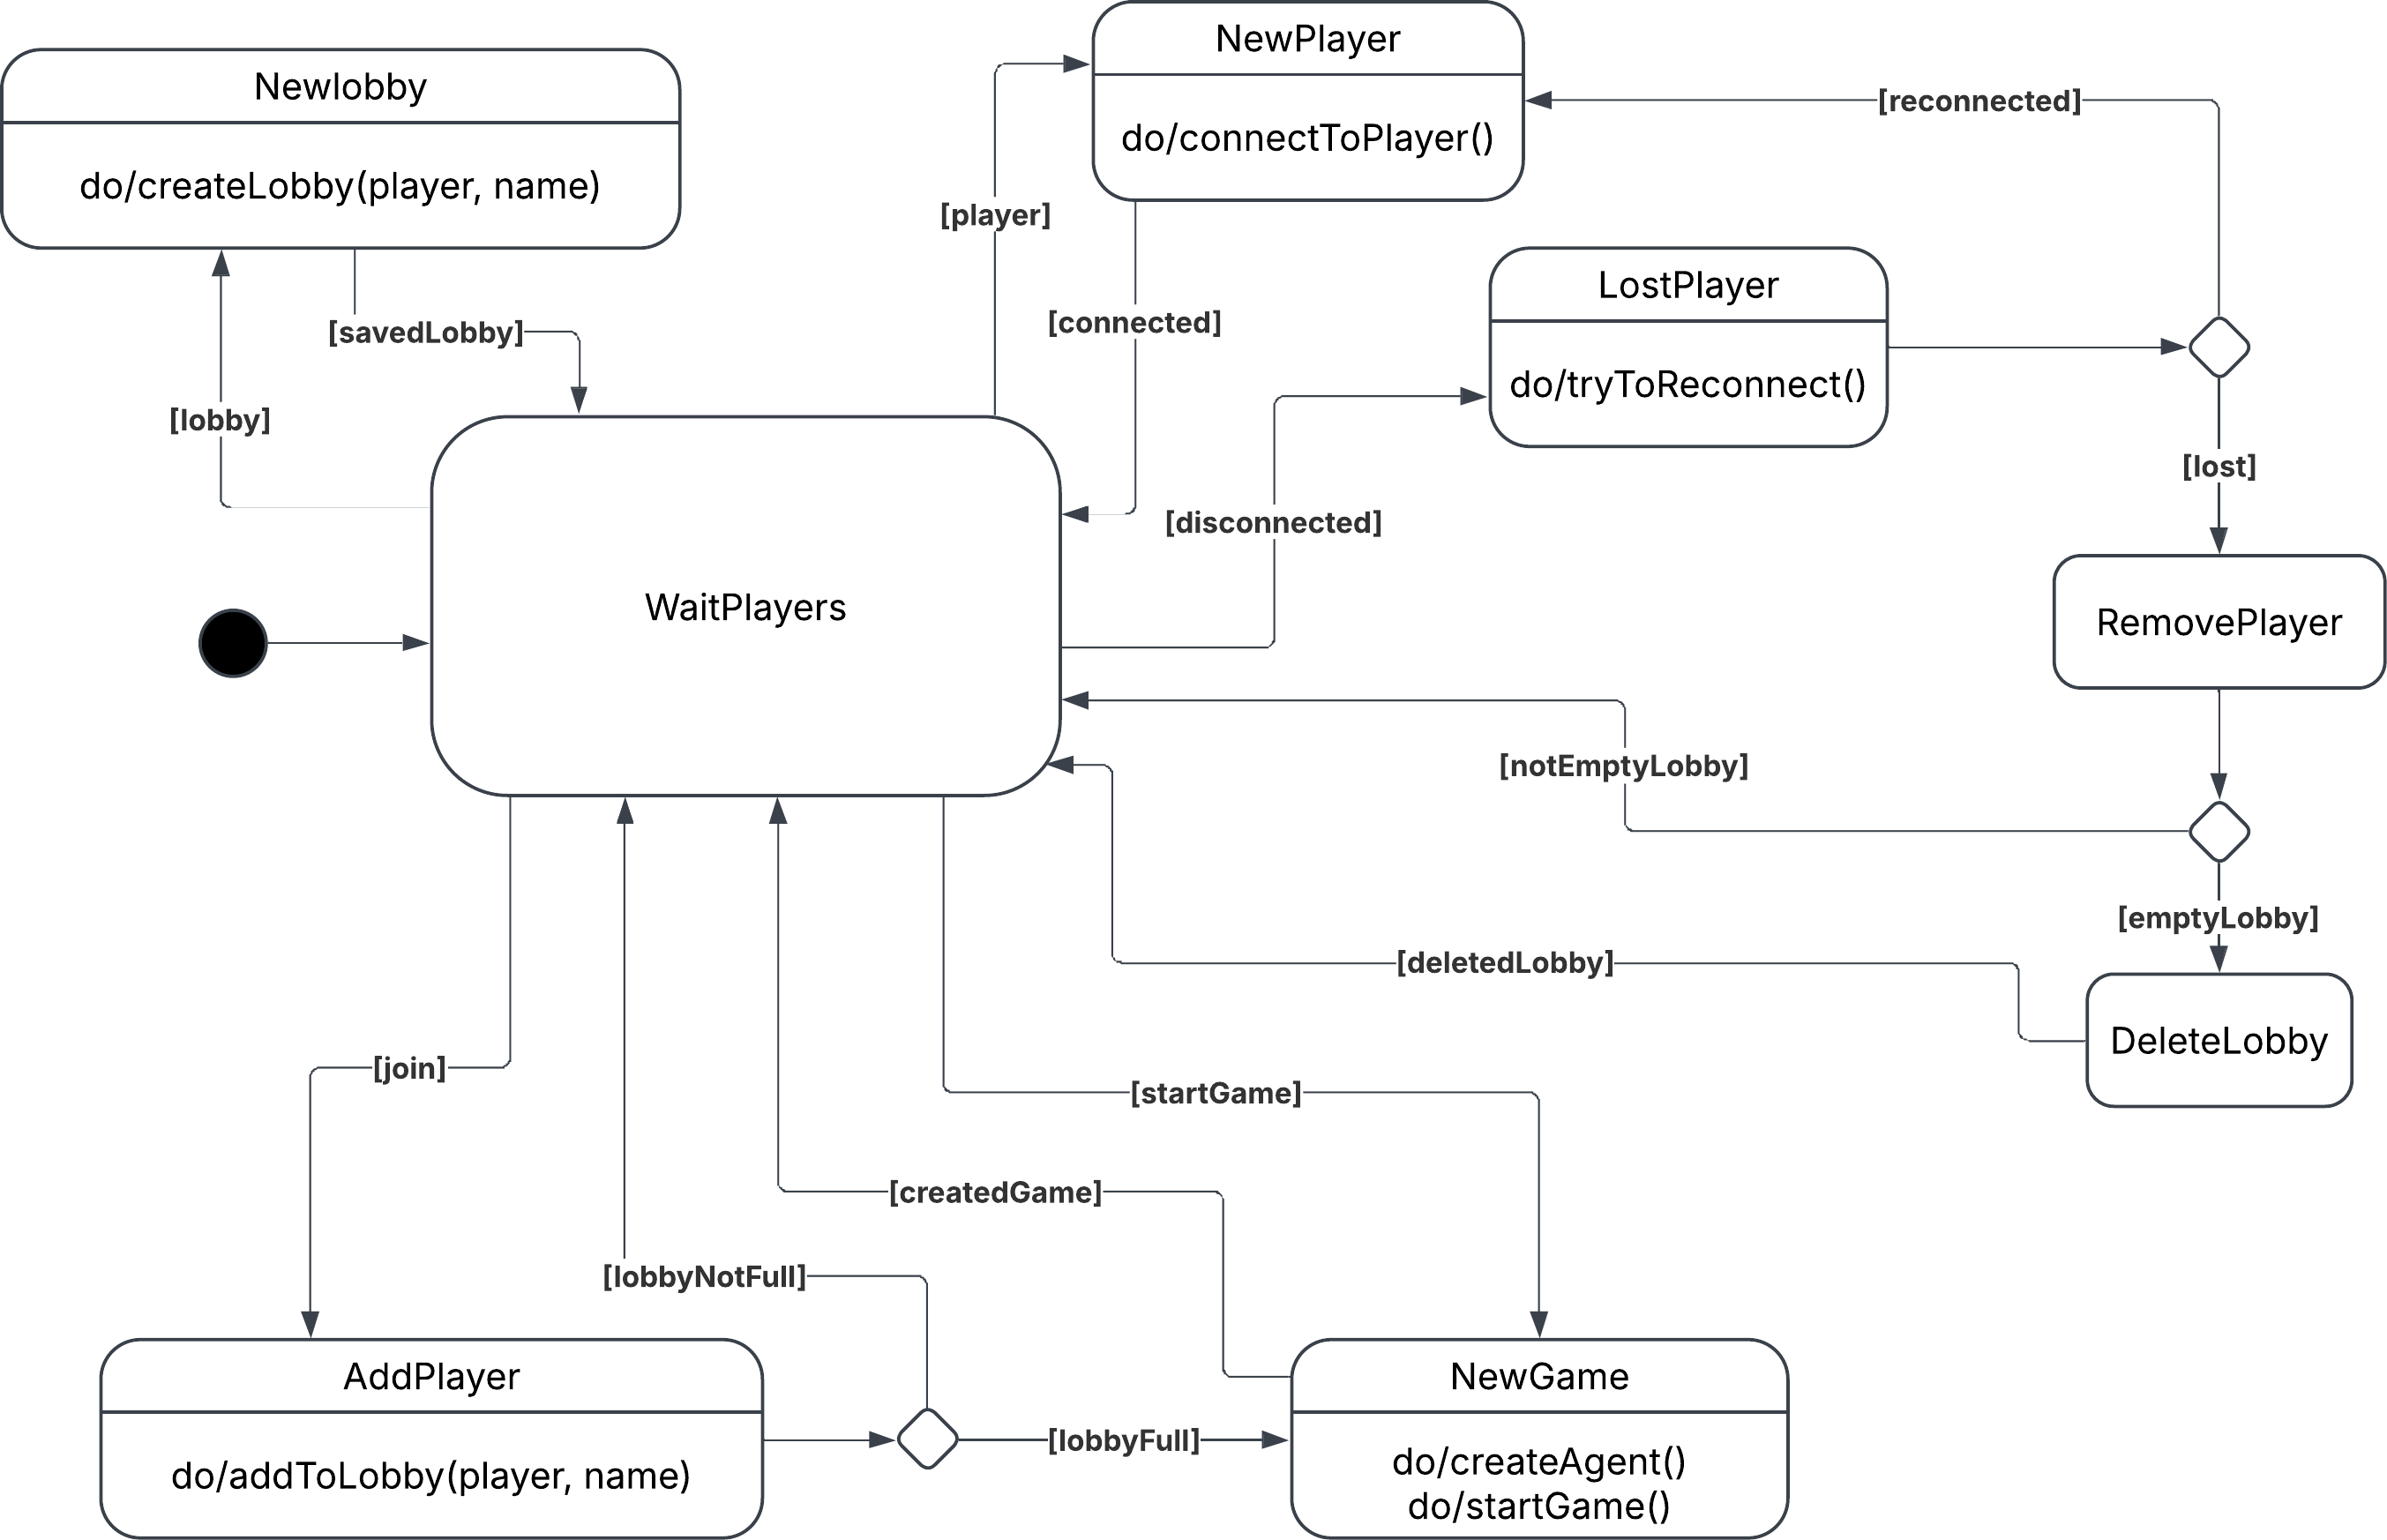
\includegraphics[width=0.8\textwidth]{figures/serverStates.png}
    \caption{State diagram of the server} 
    \label{fig:serverStates}
  \end{figure}
  \item
  \textbf{The broker} \cref{fig:brokerStates} \par
  The broker is the central core to all communications between all the components.
  Always active and using the MQTT standard.
  \begin{figure}[H]
    \centering
    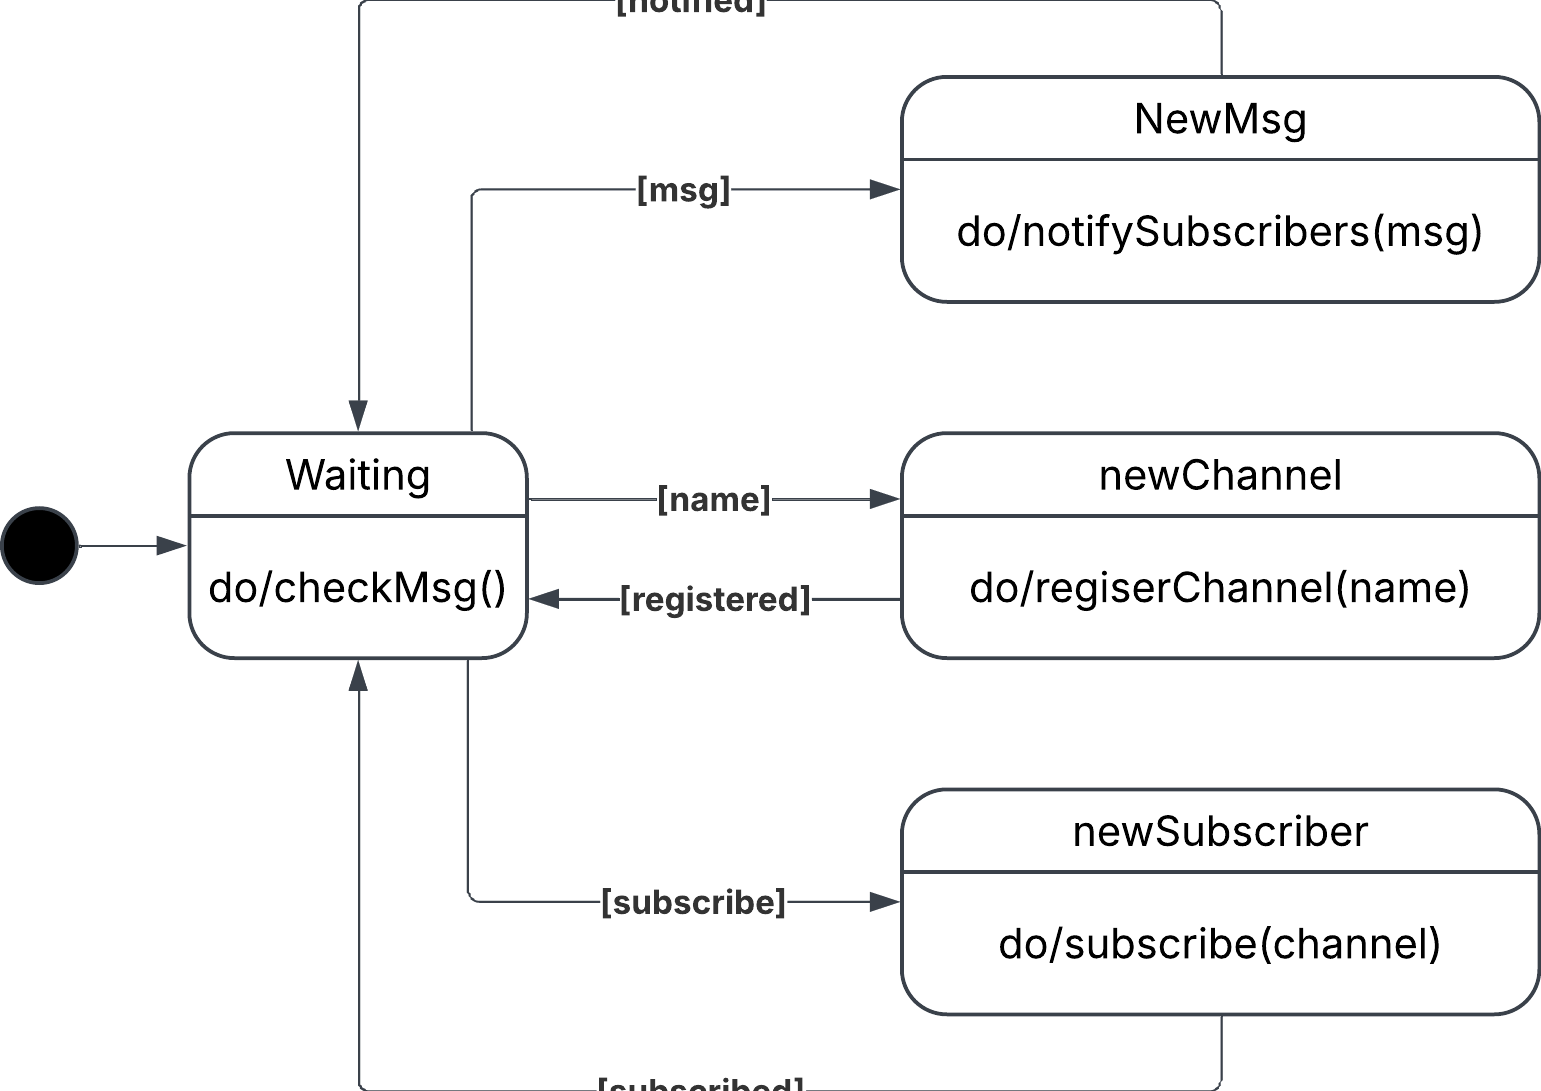
\includegraphics[width=0.8\textwidth]{figures/brokerStates.png}
    \caption{State diagram of the broker} 
    \label{fig:brokerStates}
  \end{figure}
  \item 
  \textbf{The game agent} \cref{fig:gameAgentStates} \par
  The game agent is an istance of the server that takes on the role of managing the single matches.
  It is in charge of managing the game state, the players' moves and the game logic. \newline
  It also preoccupies itself to reconnect the players and resume the game where it left off 
  in case of disconnection. Only checking each connection every time it's the player's turn to
  save some resources.
  \begin{figure}[H]
    \centering
    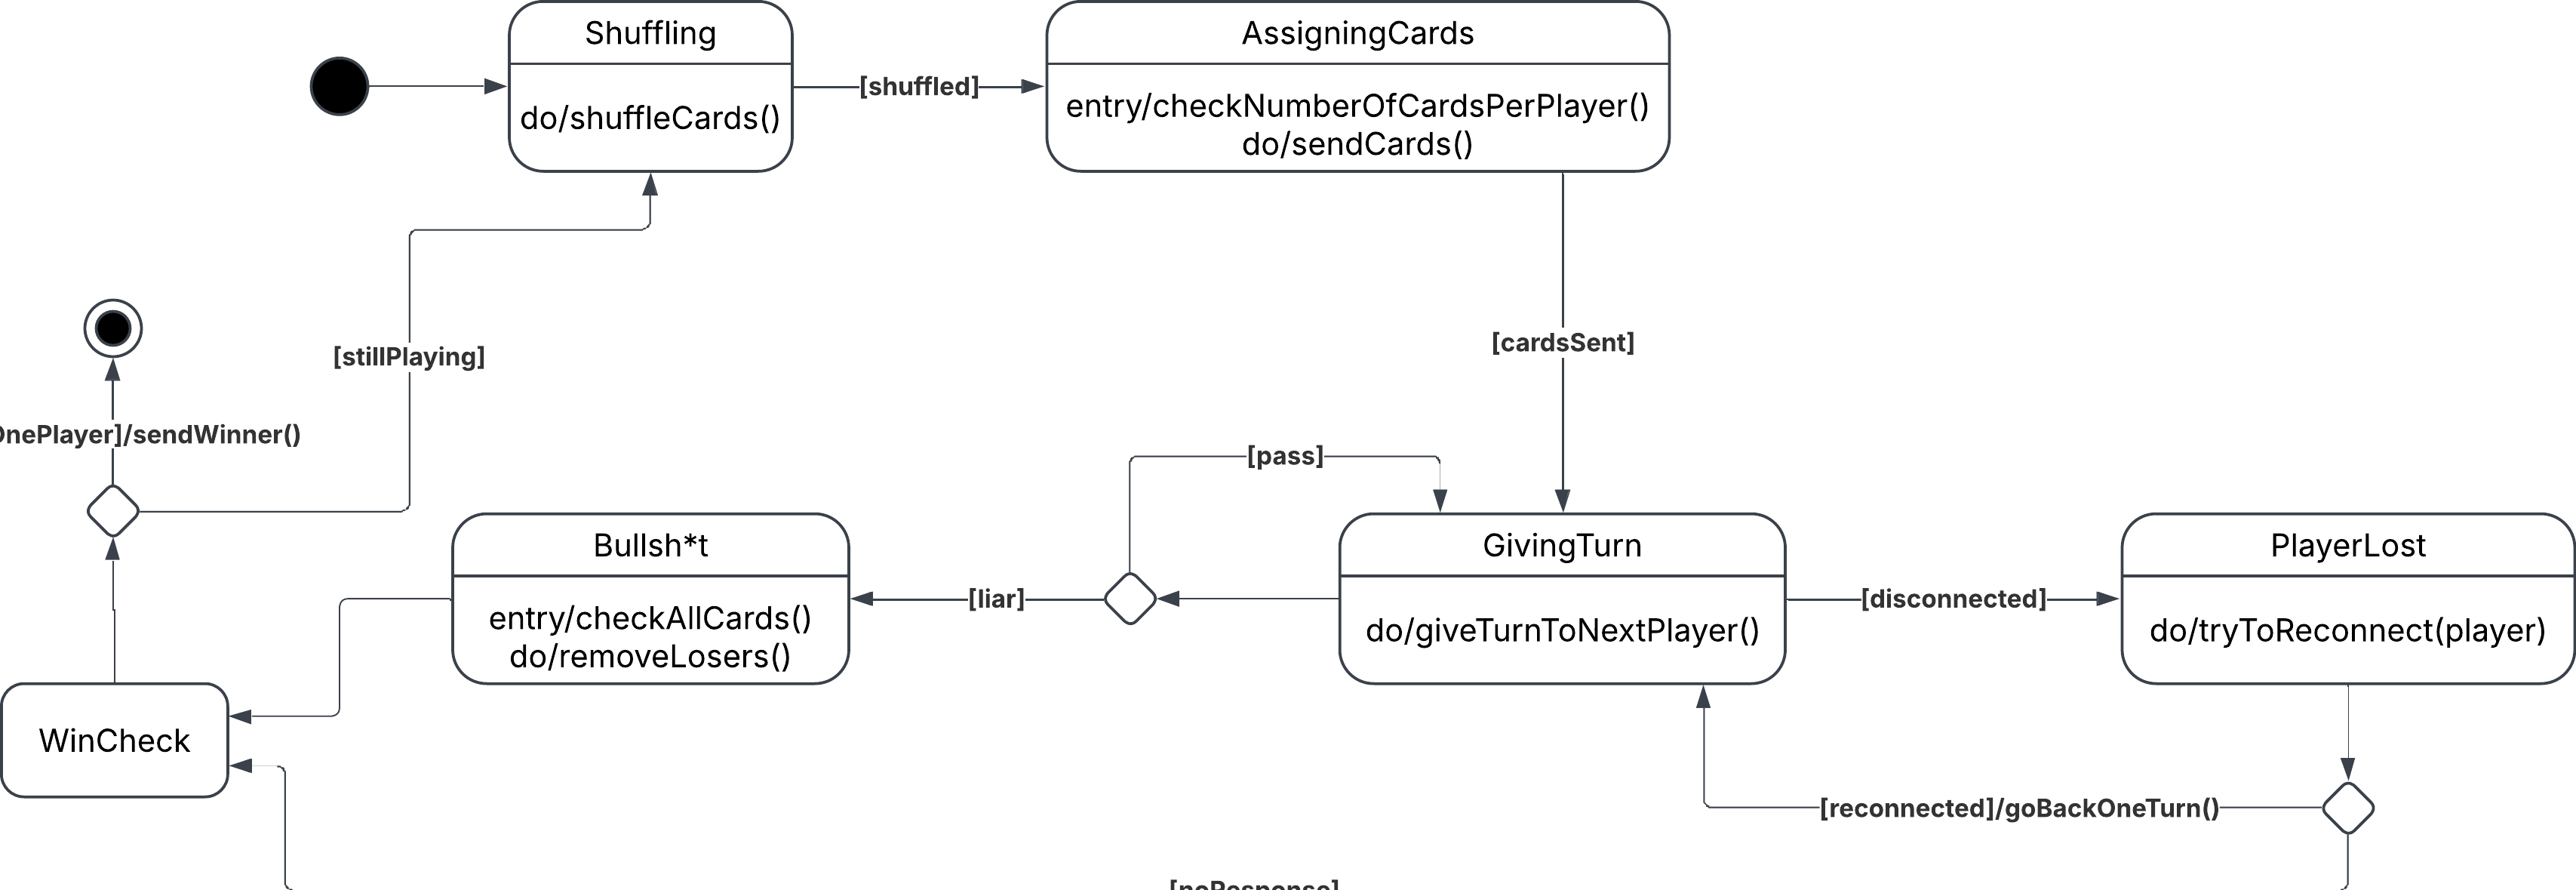
\includegraphics[width=0.8\textwidth]{figures/gameAgentStates.png}
    \caption{State diagram of the game agent} 
    \label{fig:gameAgentStates}
  \end{figure}
  \item 
  \textbf{The backup} \cref{fig:backupStates} \par
  The backup has to keep a record of every message sent by the broker, keeping a copy of server state. \newline
  This way if the server or the broker fails it can launch a new istance of whichever failed and resume 
  the service. This is a mechanism of fault tolerance that will be discussed later.
  \begin{figure}[H]
    \centering
    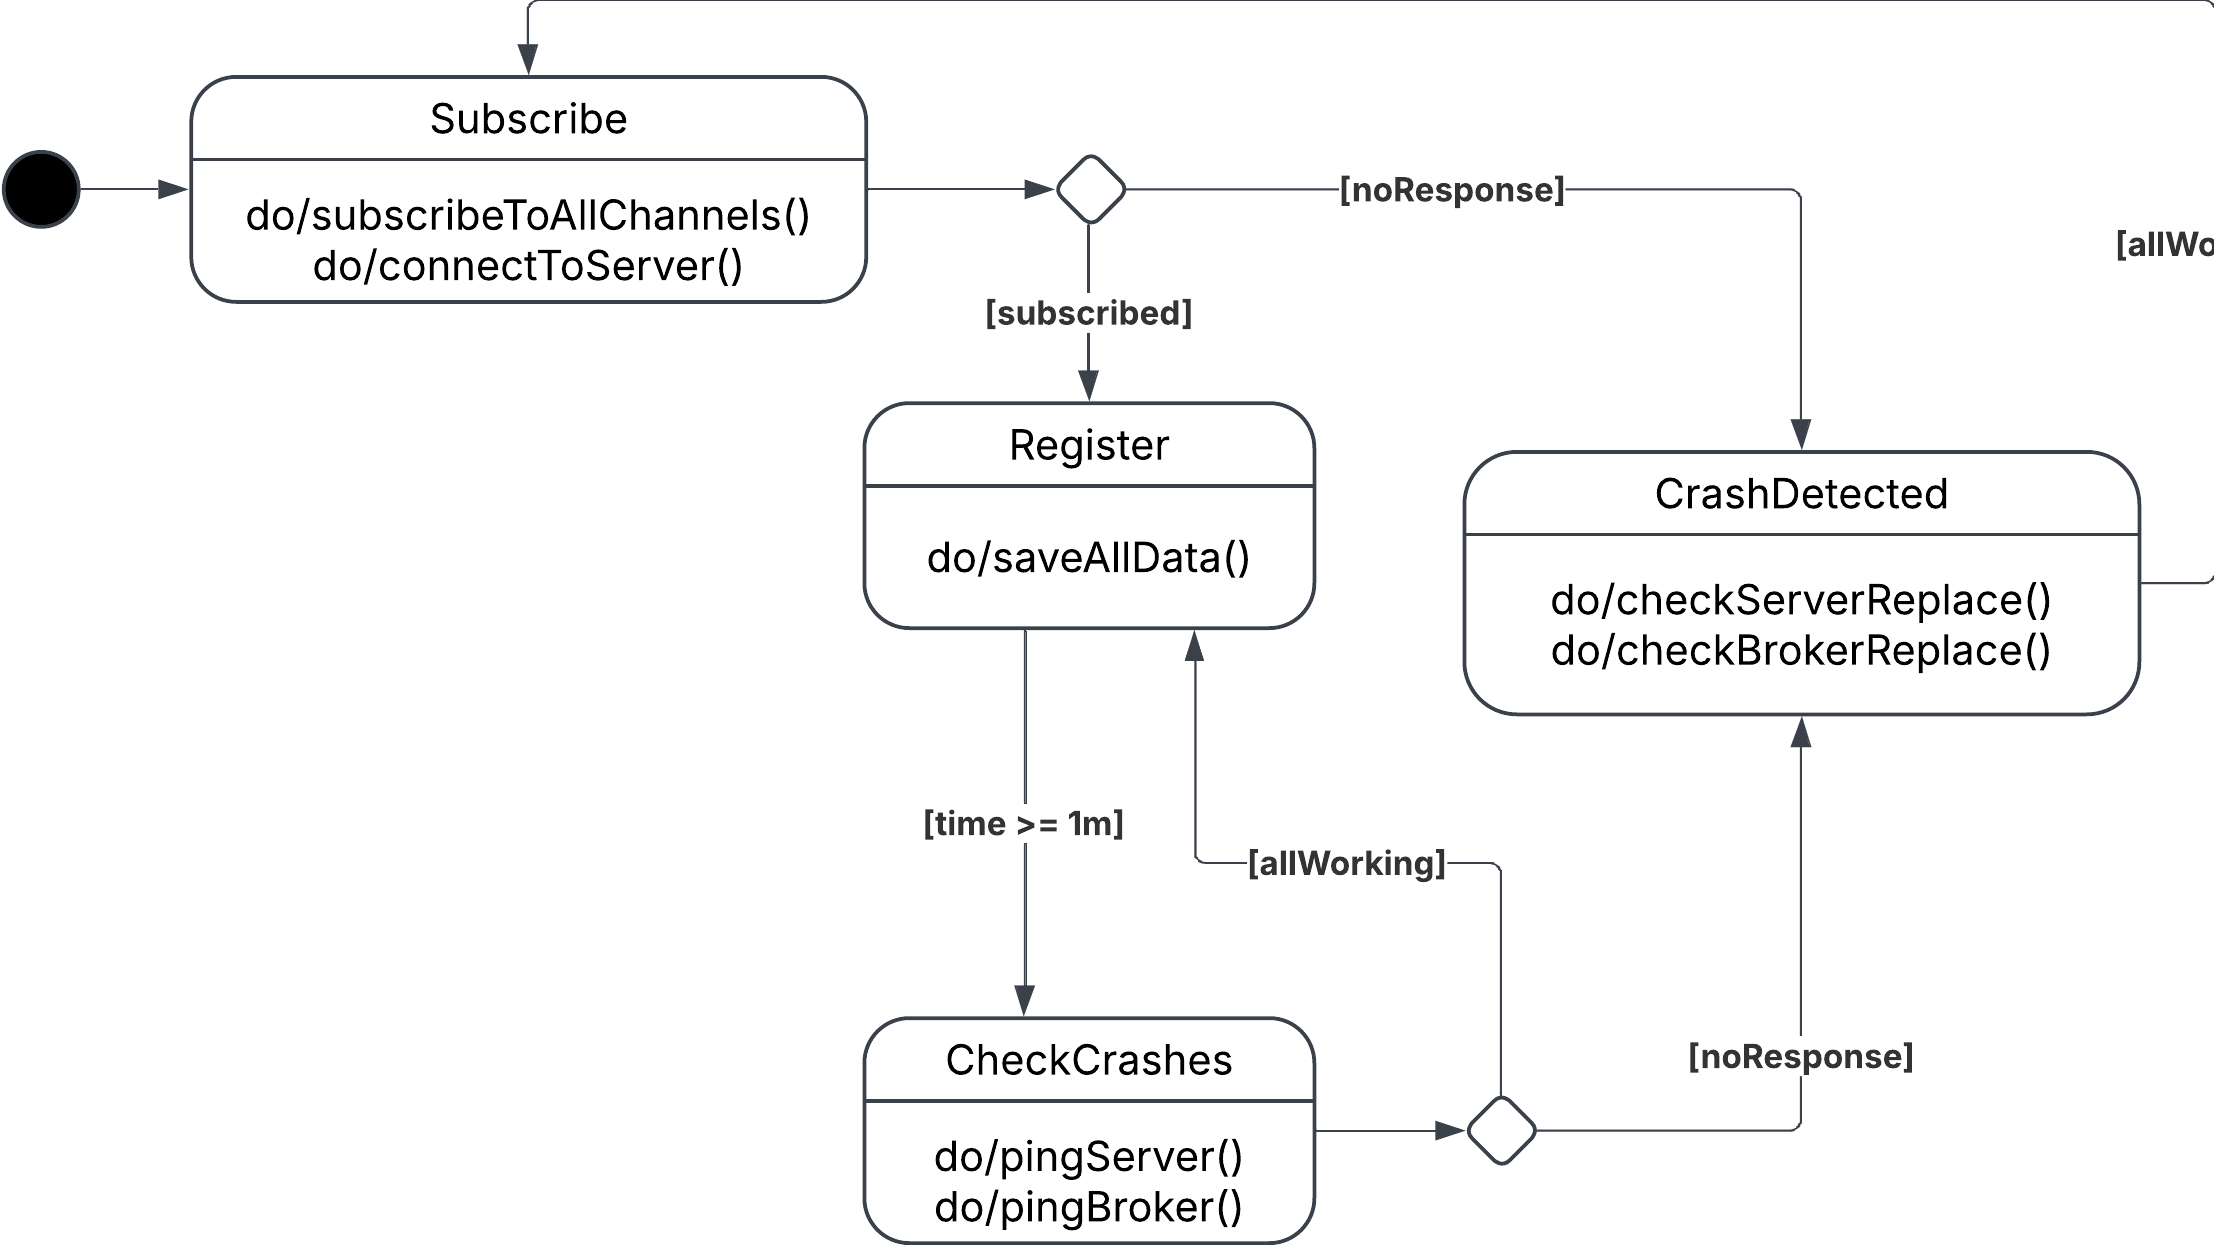
\includegraphics[width=0.8\textwidth]{figures/backupStates.png}
    \caption{State diagram of the backup} 
    \label{fig:backupStates}
  \end{figure}
\end{itemize}

\subsection{Data and Consistency
Issues}\label{data-and-consistency-issues}

Since we don't need to store data permanently because this is a card game, we don't deal with queries and databases. \newline
Some datas are shared between components, for example the game status, the players' nicknames, and other crucial information to perform the game. \newline

\subsection{Fault-Tolerance}\label{fault-tolerance}
% \begin{itemize}
%   \item Is there any form of data \textbf{replication} / federation / sharing?

%   \begin{itemize}
%     \item \emph{why}? \emph{how} does it work?
%   \end{itemize}
%   \item Is there any \textbf{heart-beating}, \textbf{timeout}, \textbf{retry
%   mechanism}?

%   \begin{itemize}
%     \item \emph{why}? \emph{among} which components? \emph{how} does it work?
%   \end{itemize}
%   \item Is there any form of \textbf{error handling}?

%   \begin{itemize}
%     \item \emph{what} happens when a component fails? \emph{why}? \emph{how}?
%   \end{itemize}
% \end{itemize}
Different types of fault tolerance are implemented in the systems, everything is set up to keep
the game running even if some components fail. \newline
The mechanics differ in their scope and purpose:
\begin{itemize}
  \item
  \textbf{Server-Side} \par
  The server and the broker are at the core of the game, if they fail the game is lost. \newline
  To prevent this from happening, they are costantly monitored.
  There are two different implementations of fault tolerance:
  \begin{itemize}
    \item \textbf{Backup Server} \par
    The server is backed up by a second server that runs as a server but is not active; so it only listens to the messages sent by the clients and the broker and keeps a copy of the game state. \newline
    If the main server fails, the backup server can take its place and resume the communication between the clients and the broker. With this mechanism, if the main server fails, the backup server can take its place and resume the system but not the game, so the game is lost.
    This happens because the \texttt{game\_loop} runs as a thread launched by the main server, so if the main server fails during a game, the game loop is lost too; so in that case, all the players receive a message that the game is over and they are redirected to the lobby screen. \newline
    This is implemented using a heartbeat mechanism, where the server sends a heartbeat message to backup server every 2 seconds. If the backup does not receive the heartbeat message within a certain time frame, it assumes that the main server has failed and takes his place elevating itself to the main server. \newline
    \item \textbf{Broker Backup} \par
    The broker is backed up by a second broker that keeps a copy of the messages sent by the clients and the server. 
    If the main broker fails, the backup broker can take its place and resume the communication between the clients and the server.
    This is implemented using the mosquitto configuration file, where the main server is configured to send a copy of every message to the backup broker with a bridge connection. \newline
    The backup broker is configured to listen to the same topics as the main broker, so it can receive the messages sent by the clients and the server. \newline
    When the main broker fails, the \texttt{ConnectionHandler} class in the client tries to reconnect to the backup broker, and if it succeeds, it can resume the communication with the server and the game. \newline
  \end{itemize}
  \textbf{Client-Side} \par
  To make sure that no accidental disconnection can ruin the game, the game agent checks the connection
  of each player every time it's their turn. If a player is disconnected, the game agent will wait for
  them to reconnect, if they don't in a certain time frame they will be kicked from the game. \newline
  Furthermore, the client always has the opportunity to try to reconnect, picking where it left
  off, if anything goes wrong.
\end{itemize}

\subsection{Availability}\label{availability}
% \begin{itemize}
%   \item Is there any \textbf{caching} mechanism?

%   \begin{itemize}
%     \item \emph{where}? \emph{why}?
%   \end{itemize}
%   \item Is there any form of \textbf{load balancing}?

%   \begin{itemize}
%     \item \emph{where}? \emph{why}?
%   \end{itemize}
%   \item In case of \textbf{network partitioning}, how does the system behave?

%   \begin{itemize}
%     \item \emph{why}? \emph{how}?
%   \end{itemize}
% \end{itemize}
At this time we don't really have an availability mechanism. \newline
The only type of caching we have is the broker that keeps the last message sent in a topic
and the backup server that keeps a copy of the game state in case of failure.

\subsection{Security}\label{security}

There aren't any security mechanisms in our project. \newline


\begin{center}\rule{0.5\linewidth}{0.5pt}\end{center}

\section{Implementation}\label{implementation}

The implementation phase is the one where the design is put into practice.
\subsection{Network Protocols}\label{network-protocols}
The main network protocol used is MQTT for the communication between the components. 
To implement the MQTT protocol we used the Paho library for Python, which is a client library for the MQTT protocol. \newline
Thanks to MQTT protocol and its path-like structure, we can easily create topics for each lobby and each player, allowing them to communicate with the server and with each other. \newline
An example of a topic structure is:
\begin{itemize}
  \item \texttt{create\_lobby} for the create lobby messages
  \item \texttt{join\_lobby} for the join lobby messages
  \item \texttt{lobby/}\textless LOBBY\_ID\textgreater\texttt{/raise\_stake} for the raise stake messages
  \item \texttt{lobby/}\textless LOBBY\_ID\textgreater\texttt{/check\_liar} for the liar detection messages
\end{itemize}

As we can see, the topics are structured in a way that allows us to easily identify the lobby and the type of message being sent. This is not always true, beacuse all the messages sent before the lobby joining are sent to the general topic, so every player can see them, but after the lobby joining, the messages are sent to the specific lobby topic. \newline
To recognize the messages in the general topic, we use a specific format for the messages, where the body contains the serialized player object. This part will be explained in more detail in the next sections. \newline

The communication is done using a class called \texttt{ConnectionHandler}, which is responsible for managing the connection to the broker and the communication with the server. That class provides methods to subscribe to topics, publish messages, and handle incoming messages. \newline
The clients are automatically subscribed to the game topics when they join a lobby, so they can receive the messages from the server. On the other hand, the server is subscribed to all the topics, so it can receive the messages from the clients and publish the game status. \newline
This is the list of all the topics used in the system: (as said before, some topics are used directly in this way while others are used with a specific lobby ID and pattern): 
\begin{itemize}
    \item \texttt{lobby}
    \item \texttt{new\_lobby}
    \item \texttt{new\_player}
    \item \texttt{ready\_to\_play}
    \item \texttt{start\_game}
    \item \texttt{join\_lobby}
    \item \texttt{leave\_lobby}
    \item \texttt{remove\_player}
    \item \texttt{start\_turn}
    \item \texttt{start\_round}
    \item \texttt{round\_loser}
    \item \texttt{game\_over}
    \item \texttt{raise\_stake}
    \item \texttt{check\_liar}
    \item \texttt{heartbeat}
    \item \texttt{server\_error}
    \item \texttt{game\_info}
\end{itemize}
\subsection{Data Formats and representations}\label{data-formats}

\begin{itemize}
  \item e.g.~JSON, XML, YAML, Protocol Buffers, etc.
\end{itemize}

\subsection{Technological details}\label{technological-details}

\begin{itemize}
  \item any particular \emph{framework} / \emph{technology} being exploited
  goes here
\end{itemize}

\section{Validation}\label{validation}

\subsection{Automatic Testing}\label{automatic-testing}
For the automatic testing we used the \texttt{unittest} framework, which is a built-in Python module for testing code. Every component of the system is tested with a set of unit tests that check the functionality of the methods and the correctness of the data. \newline
The tests are organized in a way that allows us to test each component individually, and then test the interaction between the components. \newline
Every model class has its own test file, where the methods are tested with different inputs and expected outputs. Also the class to serialize and deserialize messages is tested, to ensure that the messages are correctly serialized and deserialized. \newline
We don't have any automated tests for the integration between the components, or interaction tests by the network. To test the interaction between the components we used manual tests, for example, we created a lobby and joined it with multiple clients, then we tested the interaction between the clients and the server. \newline
To run the tests, we used the \texttt{unittest} command line interface, which allows us to run all the tests in a specific directory. The tests are run in a separate process, so they don't interfere with the main application. \newline
We develop the system in a TDD (Test Driven Development) way, so we write the tests before writing the code. This allows us to ensure that the code is correct and that the tests are passing. \newline

\begin{itemize}
  \item how were individual components \textbf{\emph{unit}-test}ed?
  \item how was communication, interaction, and/or integration among
  components tested?
  \item how to \textbf{\emph{end-to-end}-test} the system?

  \begin{itemize}
    \item e.g.~production vs.~test environment
  \end{itemize}
  \item for each test specify:

  \begin{itemize}
    \item rationale of individual tests
    \item how were the test automated
    \item how to run them
    \item which requirement they are testing, if any
  \end{itemize}
\end{itemize}

\begin{quote}
recall that \emph{deployment} \textbf{automation} is commonly used to
\emph{test} the system in \emph{production-like} environment
\end{quote}

\begin{quote}
recall to test corner cases (crashes, errors, etc.)
\end{quote}

\subsection{Acceptance test}\label{acceptance-test}

\begin{itemize}
  \item did you perform any \emph{manual} testing?

  \begin{itemize}
    \item what did you test?
    \item why wasn't it automatic?
  \end{itemize}
\end{itemize}

\section{Release}\label{release}

\begin{itemize}
  \item how where components organized into \emph{inter-dependant modules} or
  just a single monolith?

  \begin{itemize}
    \item provide a \emph{dependency graph} if possible
  \end{itemize}
  \item were modules distributed as a \emph{single archive} or \emph{multiple
  ones}?

  \begin{itemize}
    \item why?
  \end{itemize}
  \item how were archive versioned?
  \item were archive \emph{released} onto some archive repository (e.g.~Maven,
  PyPI, npm, etc.)?

  \begin{itemize}
    \item how to \emph{install} them?
  \end{itemize}
\end{itemize}

\section{Deployment}\label{deployment}

\begin{itemize}
  \item should one install your software from scratch, how to do it?

  \begin{itemize}
    \item provide instructions
    \item provide expected outcomes
  \end{itemize}
\end{itemize}

\section{User Guide}\label{user-guide}

\begin{itemize}
  \item how to use your software?

  \begin{itemize}
    \item provide instructions
    \item provide expected outcomes
    \item provide screenshots if possible
  \end{itemize}
\end{itemize}

\section{Self-evaluation}\label{self-evaluation}

\begin{itemize}
  \item An individual section is required for each member of the group
  \item Each member must self-evaluate their work, listing the strengths and
  weaknesses of the product
  \item Each member must describe their role within the group as objectively
  as possible.
\end{itemize}

It should be noted that each student is only responsible for their own
section
\bibliographystyle{plain}
\bibliography{references}
\cite{adams1995hitchhiker} % Example citation to avoid the no citation error



\end{document}
